\subsection{Iteration \#2}
I iteration 2 udvides systemet, så bruger kan logge på webapplikationen og lave flyveopsætninger, som dronen skal flyve efter. Funktionaliteten af webapplikationen udvides, så det bliver muligt at lave flyveopsætninger. Når en flyveopsætning er lavet, skal den gøres tilgængelig for dronen, hvilket kræver tilføjelser i kommunikationen mellem drone og server. 
Desuden skal dronen finde egen GPS position, flyvehøjde og orientering. Ud fra viden om egen position, flyvehøjde og orientering skal dronen flyve til de lokationer som er fastsat i flyveopsætningen. 


\subsubsection*{User story}
Bruger logger på webapplikationen med sit brugernavn og password. Når der er logget korrekt ind vises bruger sin eller sine droner på en liste. Ved at trykke på en drone vises bruger information om den pågældende drone. Informationen består af waypoints, om der skal tages billeder ved de forskellige waypoints samt indstilling af flyvehøjde. Bruger klikker på en drone fra listen og klikker derefter på kortet for at tilføje waypoints som tilsammen udgør et event. Bruger tildeler eventet navn og en kommentar og trykker "publish to drone".
Når en drone er tændt og færdig initialiseret fortæller den server om sin nuværende position og kontrollerer om en ny flyveopsætning er tilgængelig. Er der en ny flyveopsætning tilgængelig hentes den og dronen påbegynder flyvning.

%kommentar
\begin{figure}[H]
	\centering
	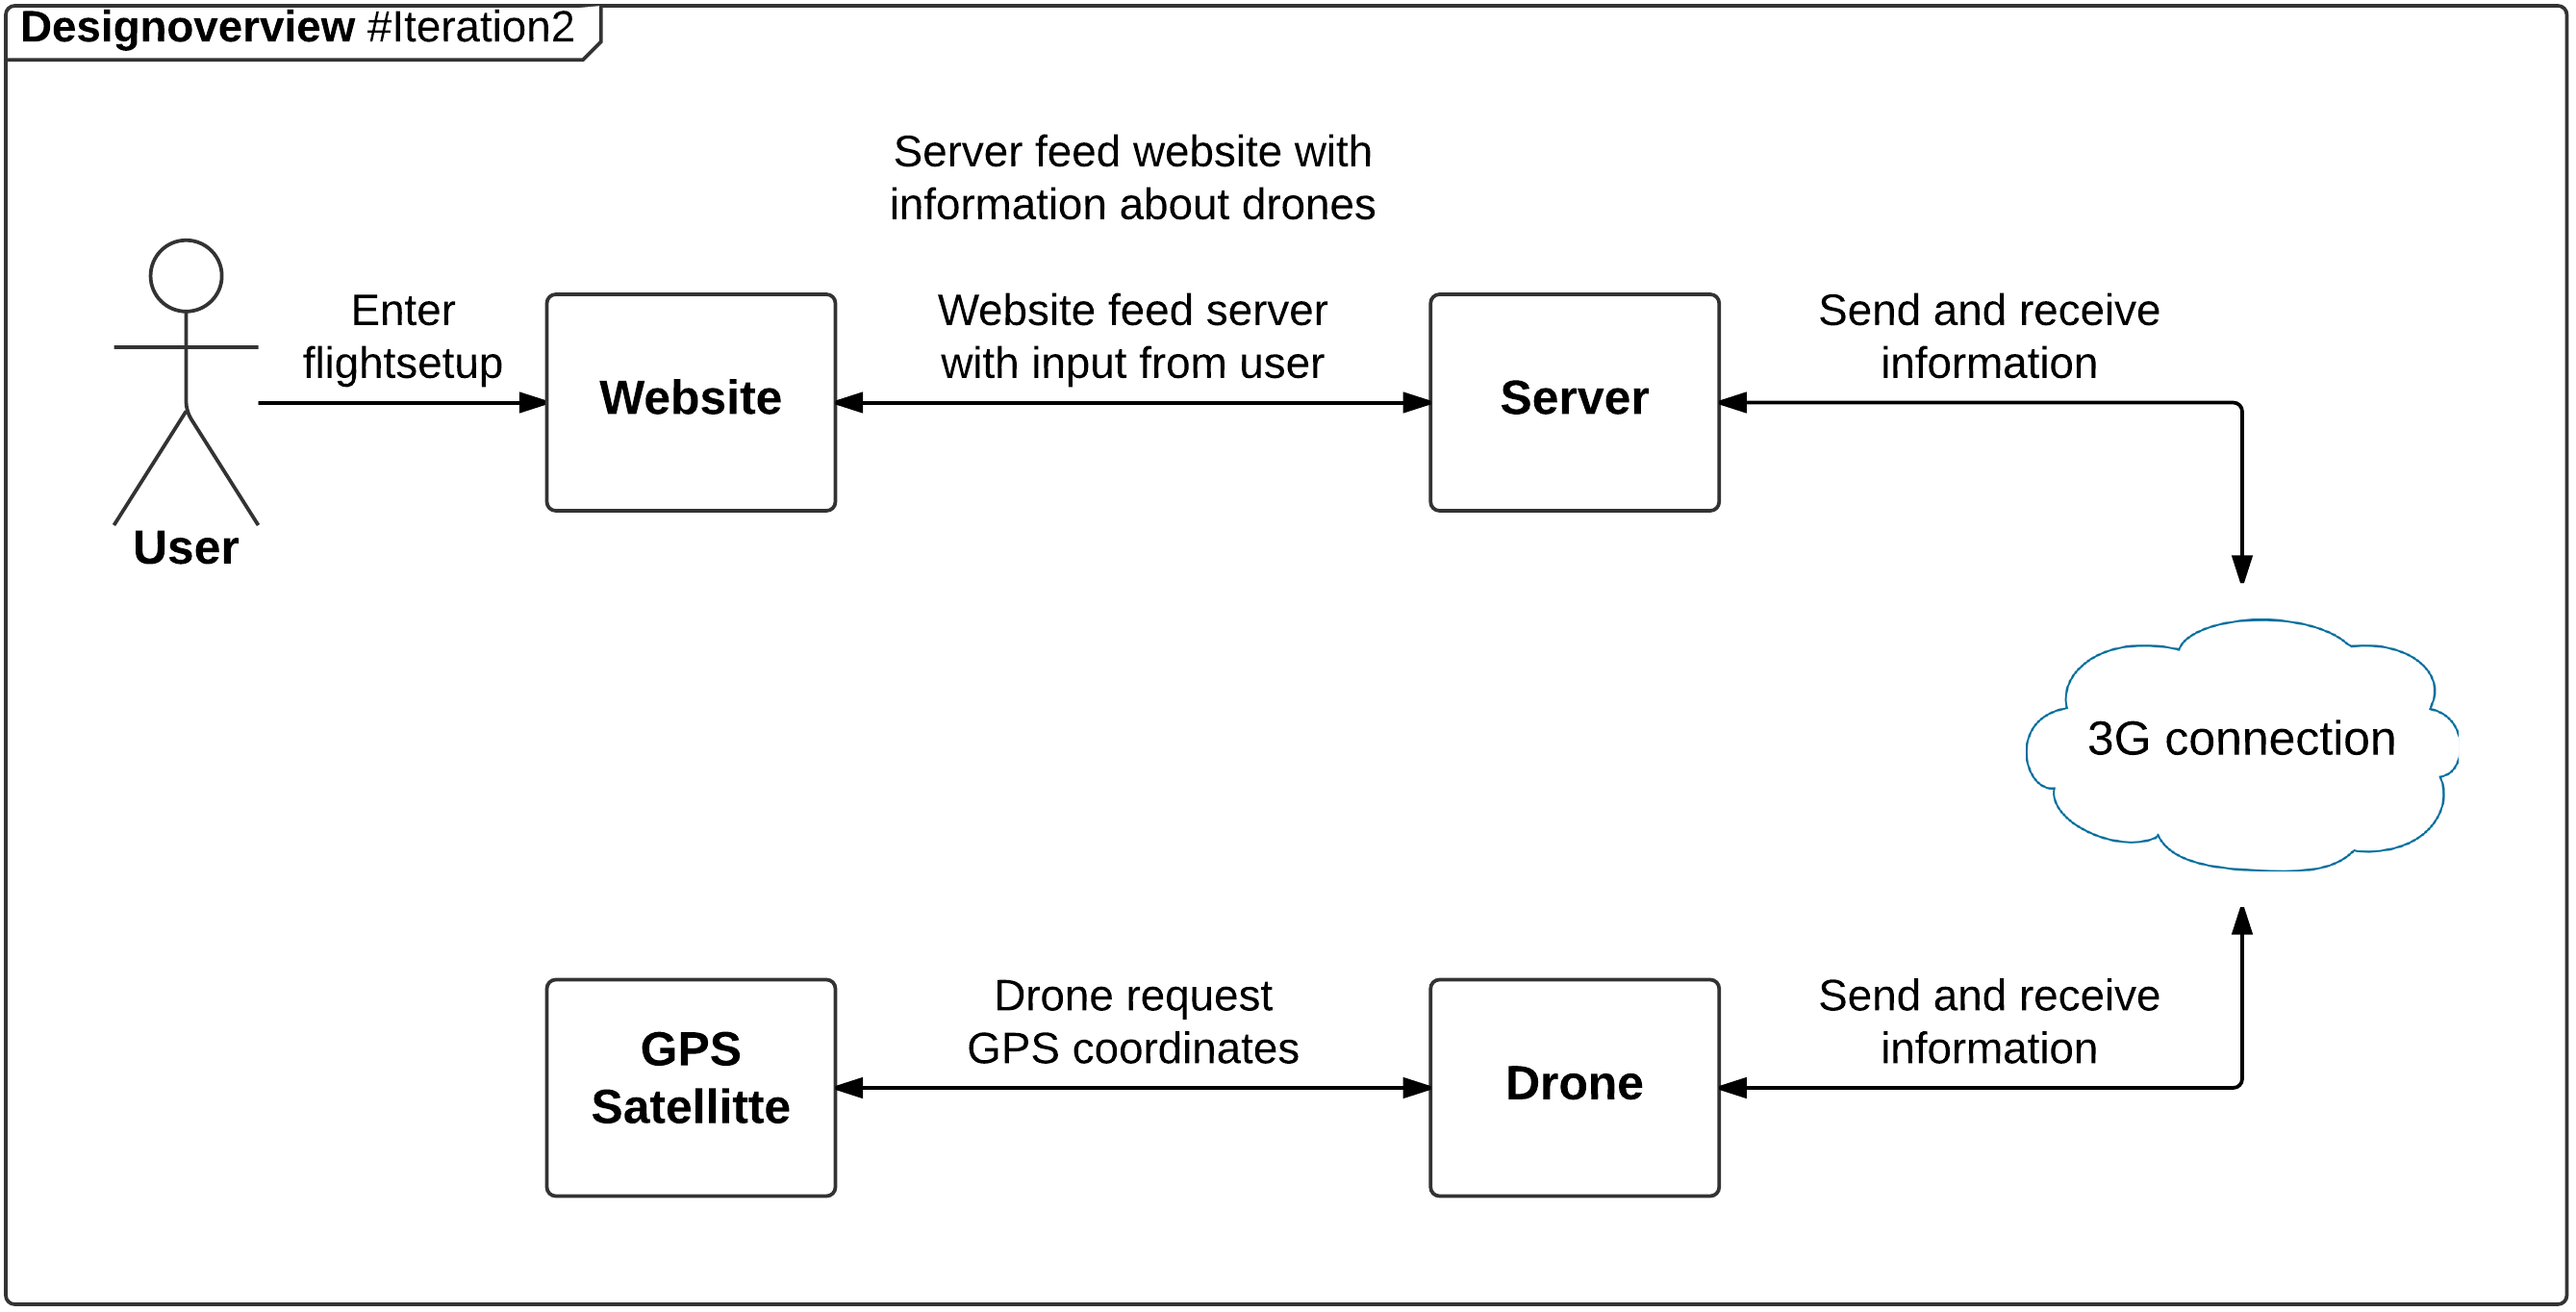
\includegraphics[width=1\textwidth]{Billeder/design_overview/design_overview_iteration2.png}
	\vspace{-.5cm}
	\caption{Designoverview \#iteration 2}
	\label{fig:design_overview_UC1}
\end{figure}


\newpage
\subsubsection*{Pakkediagram drone}
I dette afsnit vises pakkediagram tilhørende drone. De pakker der vises i pakkediagrammet består af en eller flere klasser, der med stort samspil udfører opgaver indenfor et fælles ansvarsområde. På hver pakke findes en lille beskrivelse, der tydeliggør pakkens ansvarsområde. 

\begin{figure}[H]
	\centering
	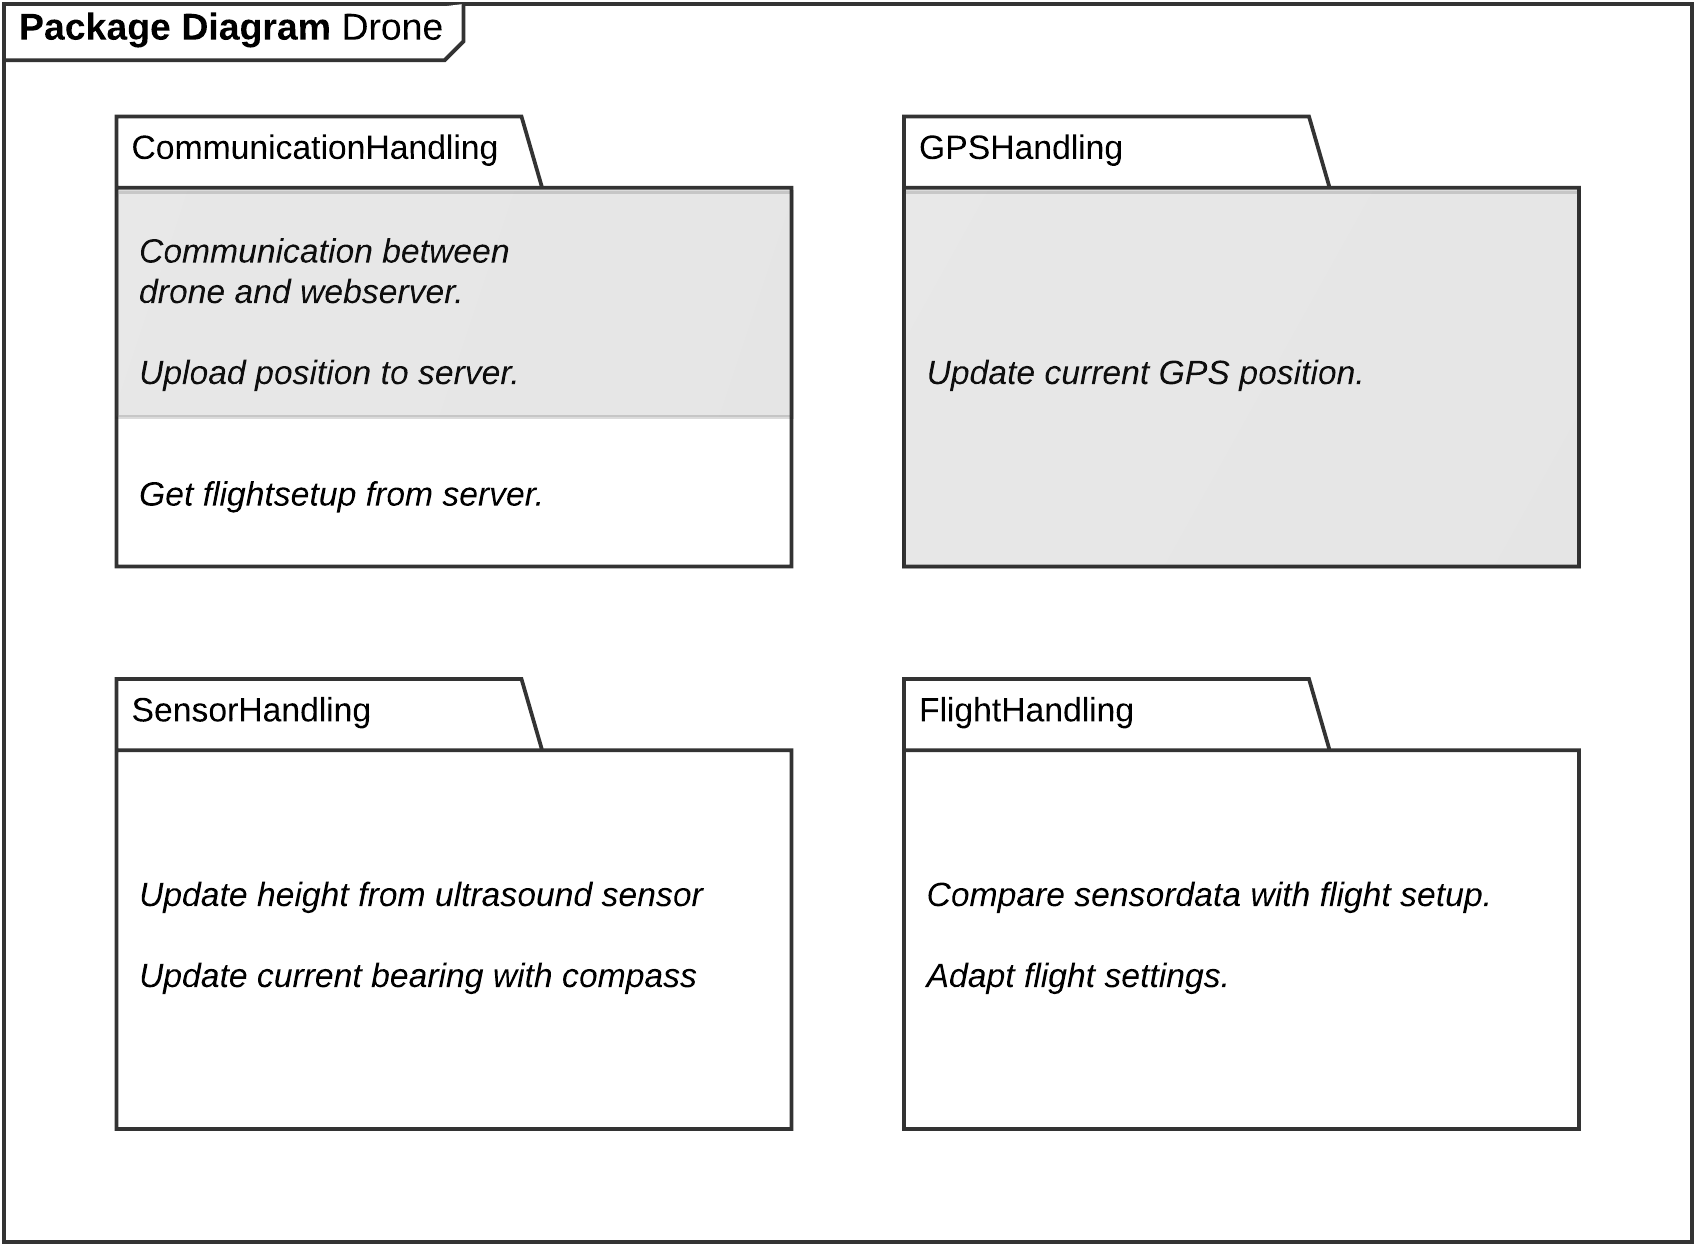
\includegraphics[width=1\textwidth]{Billeder/pakke_diagrammer/iteration2_drone.png}
	\vspace{-0.5cm}
	\caption{Pakkediagram drone}
	\label{fig:iteration2_pakke_diagram_drone}
\end{figure}

\textbf{CommunicationHandling}\\
Pakkens ansvar er kommunikation imellem drone og server. Efter denne iteration skal dronen både kunne hente flyveopsætninger fra server og sende sin nuværende GPS position til server.

\textbf{GPSHandling}\\
Pakkens ansvar er håndtering af GPS. Dels er pakken ansvarlig for opstart og initiering af GPS, og desuden bruges pakken hver gang dronens nuværende GPS position skal opdateres.

\textbf{SensorHandling}\\
Pakken er ansvarlig for indsamling af sensor data. I denne iteration skal pakken bruges til aflæsning af højdemåler og kompasset på flight control boardet. 

\textbf{FlightHandling}\\
Pakkens ansvar er kontrol og styring af drone under flyvning. Ved sammenligning af sensor data og data fra flyveopsætning tilpasses flyvehøjde, orientering mm



\newpage
\subsubsection*{Pakkediagram webapplikation}

I dette afsnit vises pakkediagram tilhørende webapplikation. De pakker der vises i pakkediagrammet består af en eller flere klasser, der med stort samspil udfører opgaver indenfor et fælles ansvarsområde. På hver pakke findes en lille beskrivelse, der tydeliggør pakkens ansvarsområde. De dele af pakkerne der er gråskraveret, er funktionalitet udarbejdet i tidligere iteration.

\begin{figure}[H]
	\centering
	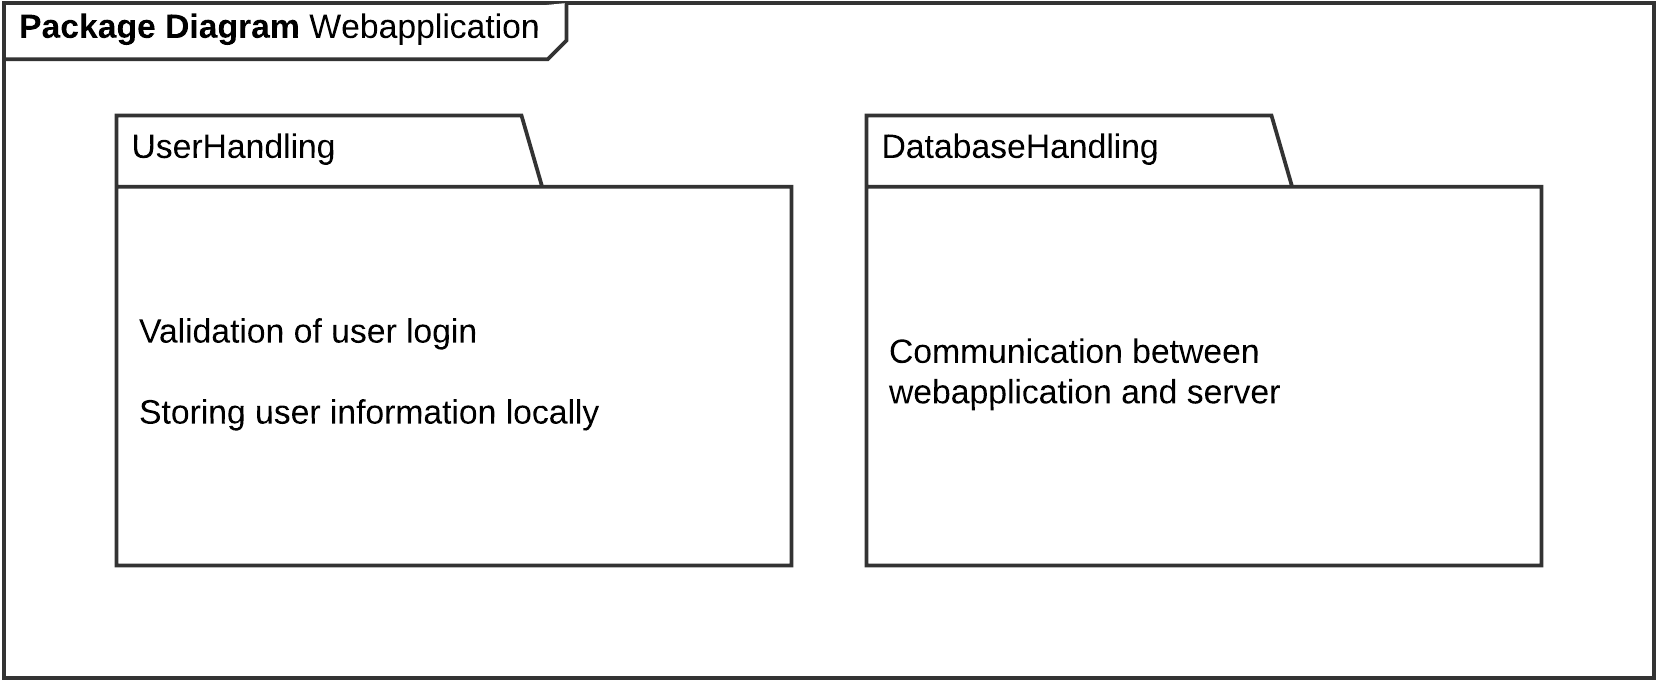
\includegraphics[width=1\textwidth]{Billeder/pakke_diagrammer/iteration1_server.png}
	\vspace{-0.5cm}
	\caption{Pakkediagram webapplikationen}
	\label{fig:iteration1_pakke_diagram_webapp}
\end{figure}

\textbf{UserHandling}\\
Pakkens ansvar er validering af login/log ud på websitet. Pakken har også ansvaret for at hente og gemme data om de forskellige brugere.

\textbf{DatabaseHandling}\\
Pakkens ansvar er kommunikation imellem databasen og serveren. 

\textbf{DroneHandling}\\
Pakken er ansvarslig for håndtering af events, waypoints og forskellige droner.

\newpage

\subsubsection*{Sekvensdiagram drone}

Til iteration 2 er systemsekvensen for drone beskrevet med flere mindre sekvensdiagrammer i stedet for et stort. Denne fremstilling gør det muligt at repræsentere systemets funktionalitet på mere overskuelig vis, hvilket bør øger forståelsen af diagrammerne. Det første sekvens diagram beskriver kommunikation mellem main controller, 3G og server. Det næste går mere i dybden med 3G modulet og underliggende klasser. Det sidste diagram viser hvordan dronen agerer under flyvning.


Af figur \ref{fig:Sekvens_diagram_iteration2_2} fremgår det hvordan dronens main controller via 3G-shieldet kommunikerer med serveren for at kontrollere om en ny flyveopsætning er tilgængelig. Når en flyveopsætning sættes tilgængelig hentes den af dronen. 

%kommentar
\begin{figure}[H]
	\centering
	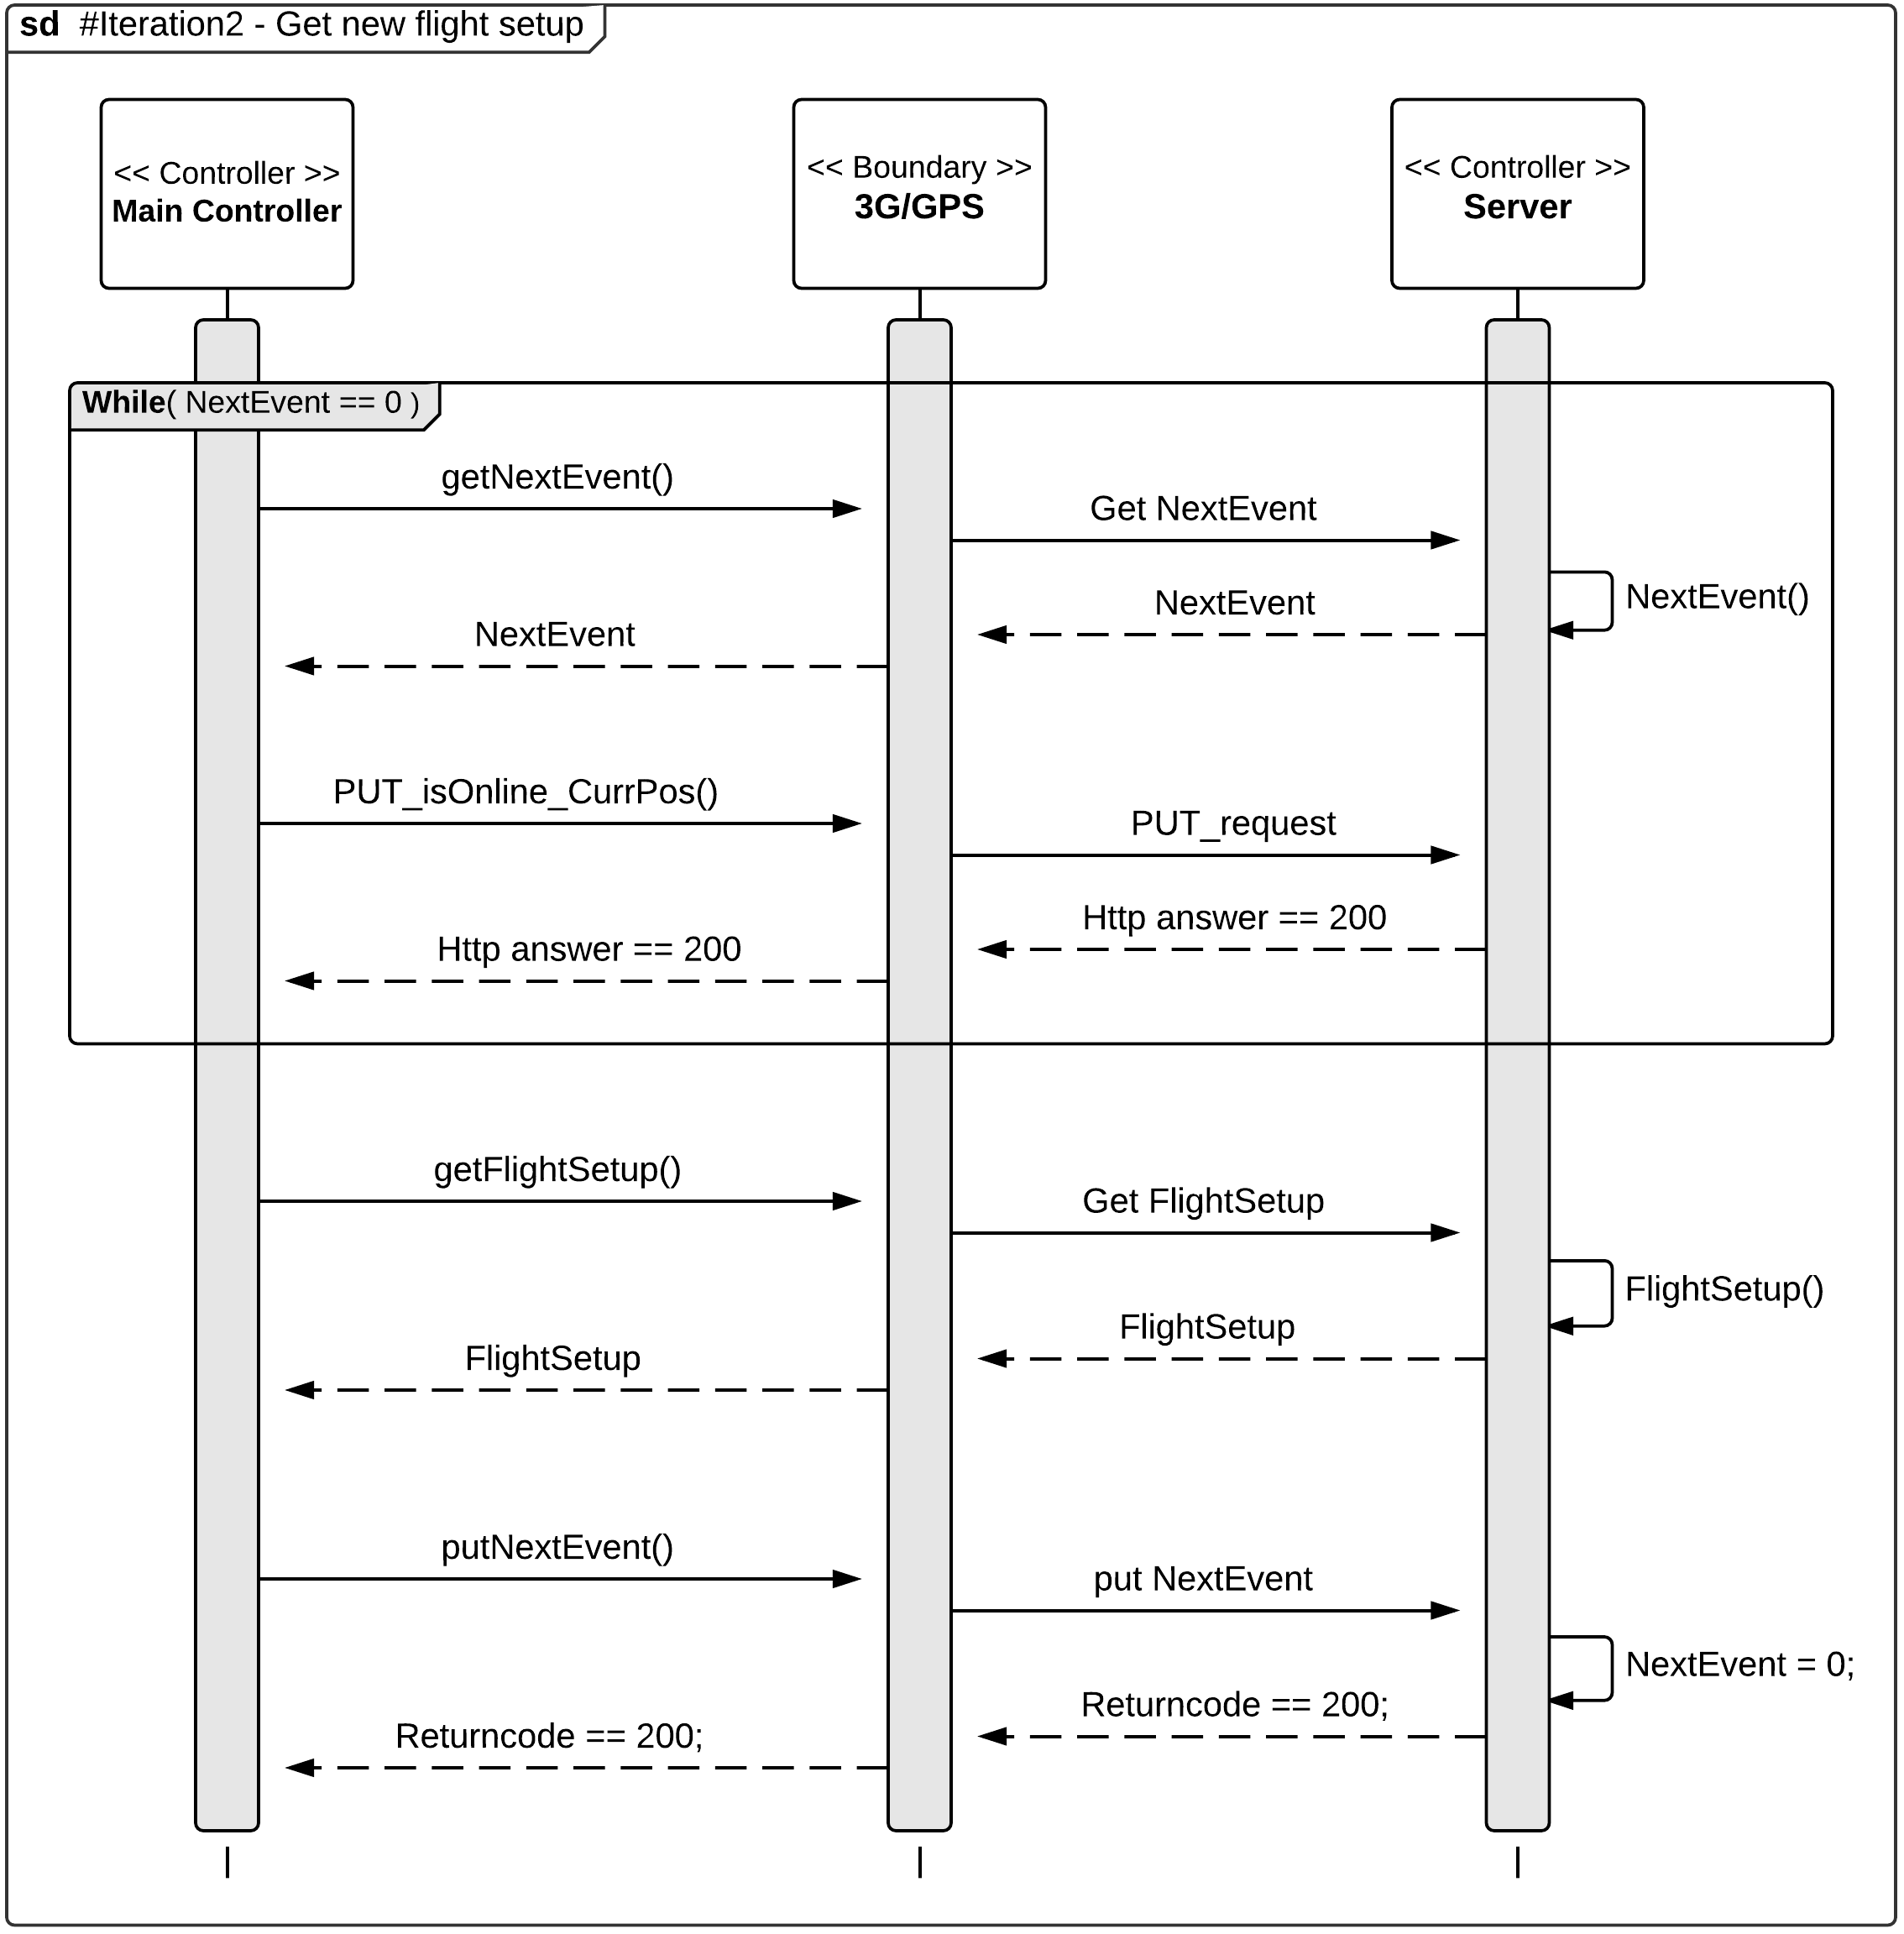
\includegraphics[width=1\textwidth]{Billeder/sekvens/sekvens_iteration2_2}
	\caption{Sekvensdiagram - hent flyveopsætning}
	\label{fig:Sekvens_diagram_iteration2_2}
\end{figure}

\newpage

Sekvensdiagrammet på figur \ref{fig:Sekvens_getwaypoints} viser en mere detaljeret beskrivelse af hvordan 3G og underliggende klasser fungerer. 3G og de underliggende klasser håndterer al kommunikation mellem drone og server.

\begin{figure}[H]
	\centering
	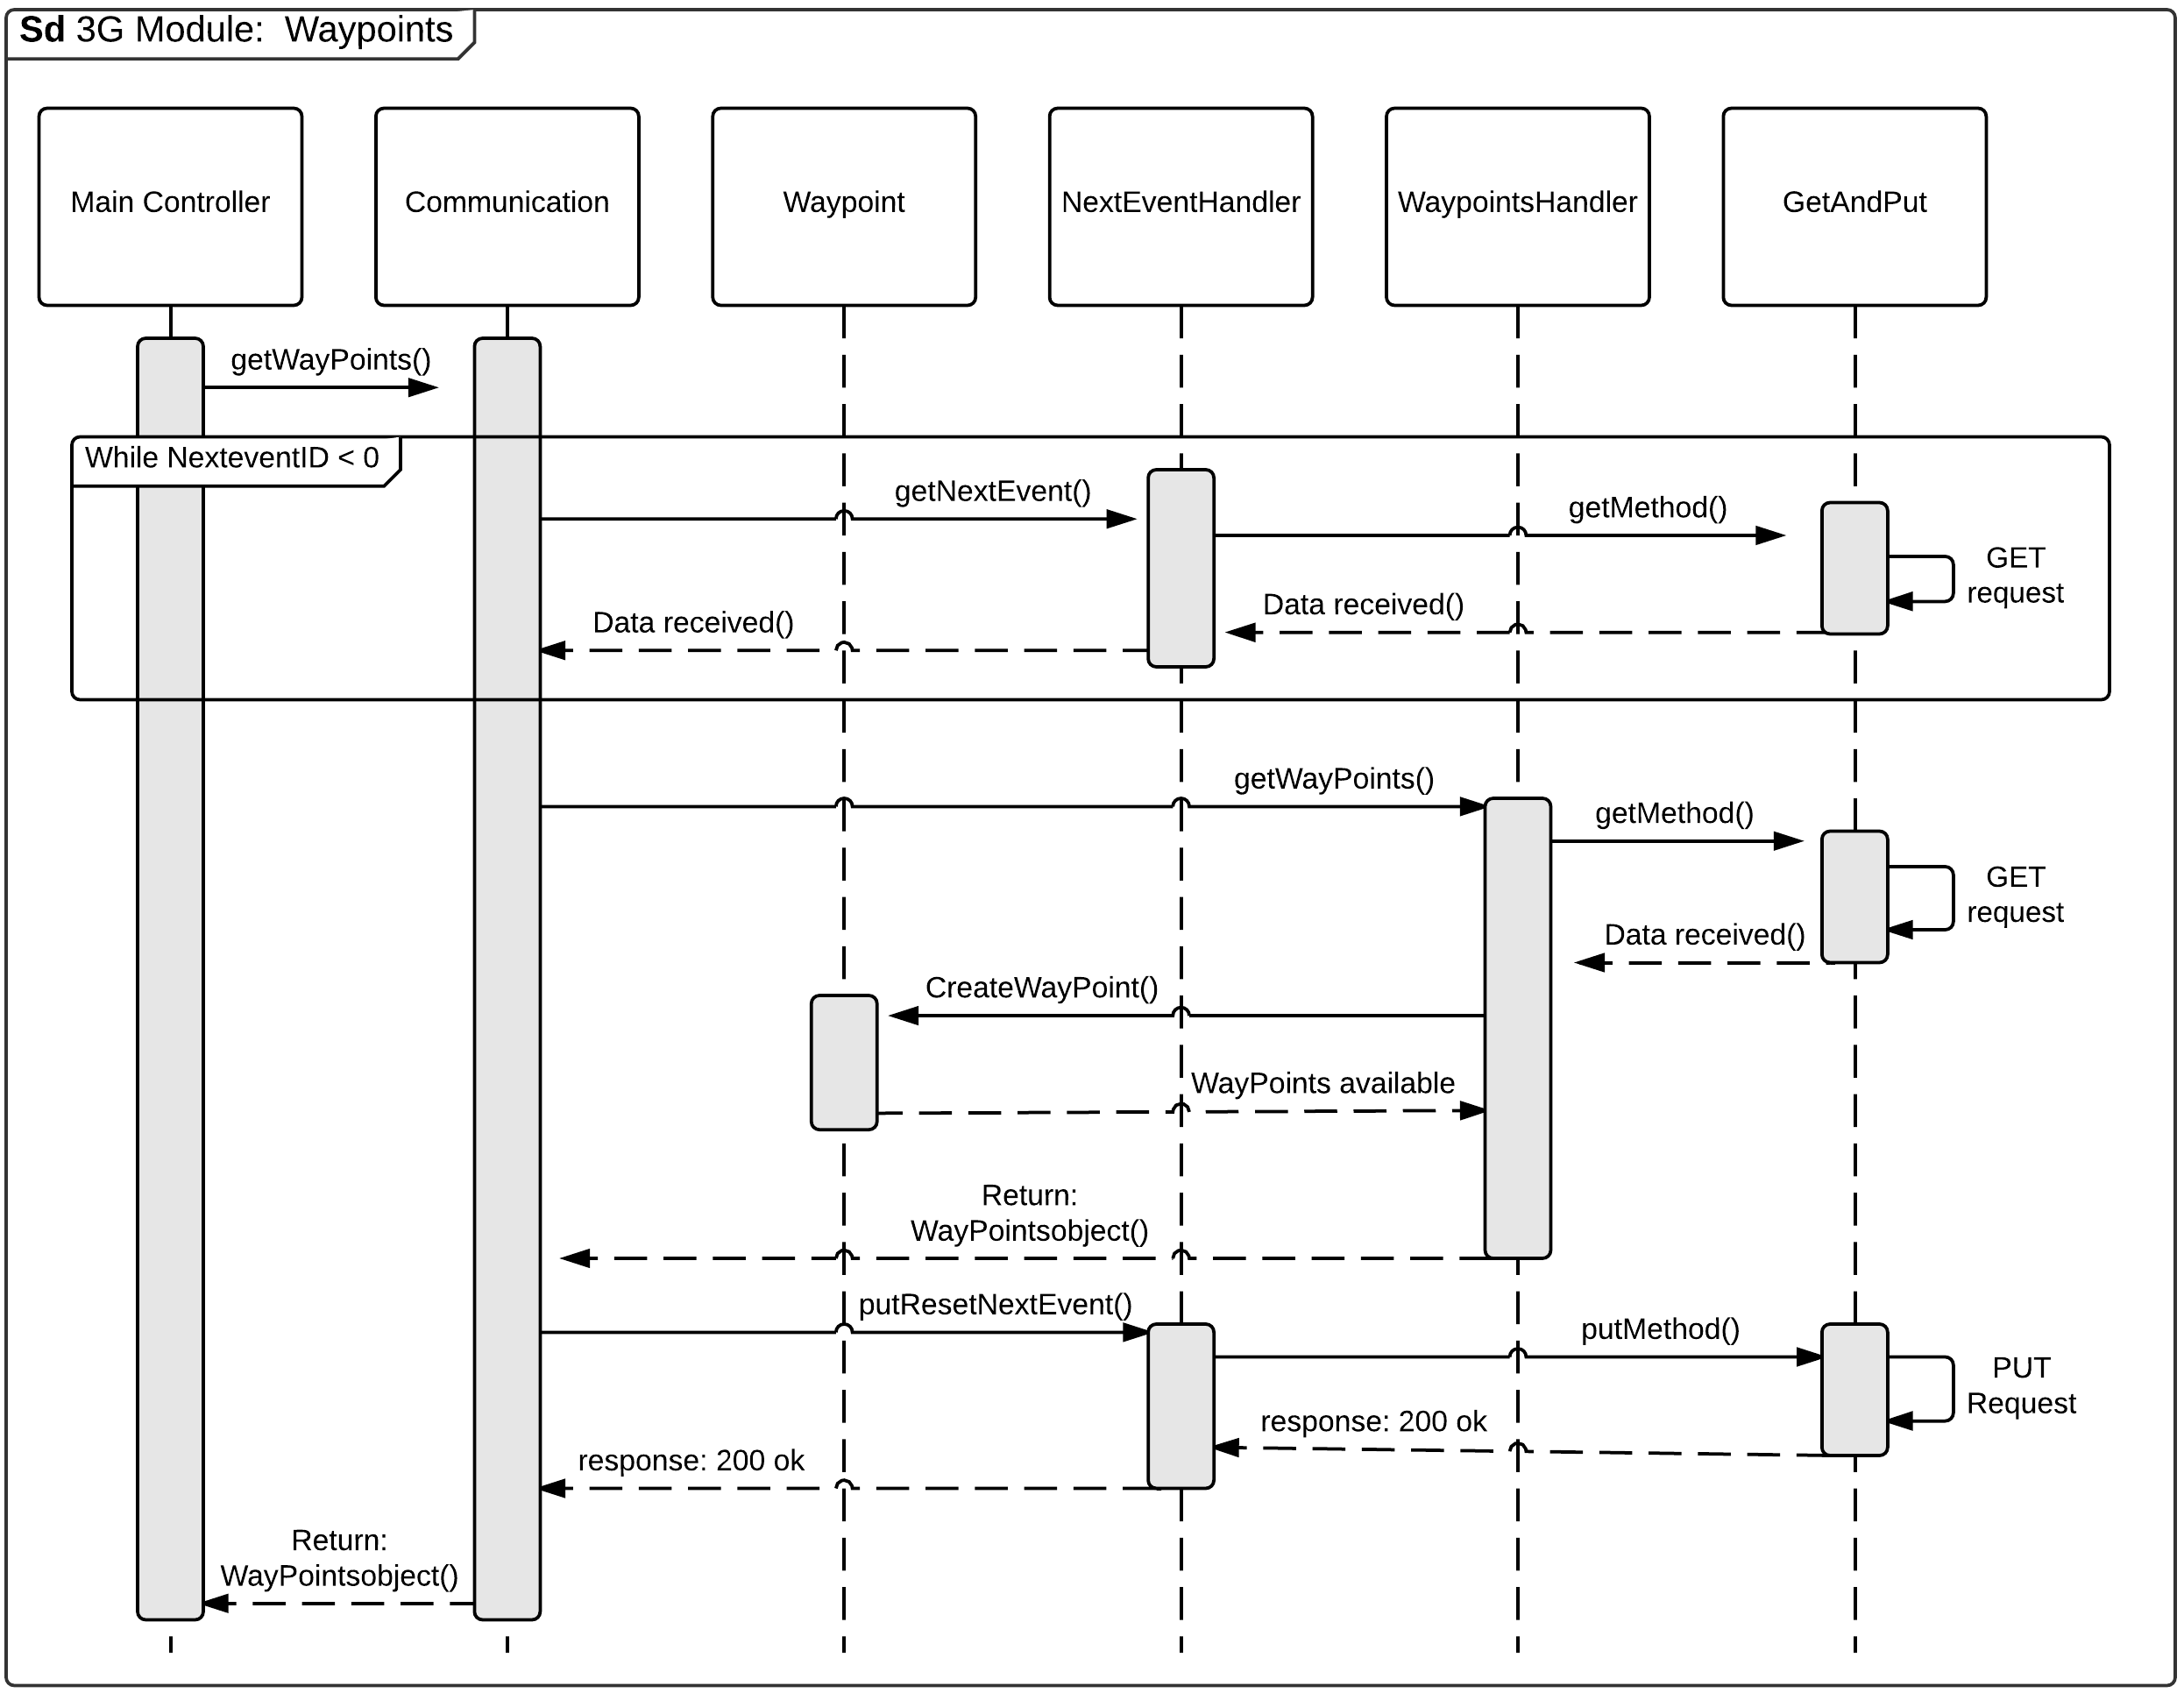
\includegraphics[width=1\textwidth]{Billeder/sekvens/sekvens_getwaypoints.png}
	\caption{Sekvensdiagram - Detaljeret kommunikation}
	\label{fig:Sekvens_getwaypoints}
\end{figure}

\newpage

Af figur \ref{fig:Sekvens_diagram_iteration2_3} fremgår det hvordan dronen agerer når den flyver autonomt mod en given GPS position. Main controlleren indsamler kompas data fra flight control boardet, latitude og longitude fra GPS og flyvehøjde fra ultralyds sensor. De indhentede data processeres og bruges til at korrigere og optimere de nuværende flyveindstillinger.
Som det fremgår af while loopet fortsætter flyvningen indtil dronen er tilpas tæt på den GPS destination bruger valgte i flyveopsætningen. 


%kommentar
\begin{figure}[H]
	\centering
	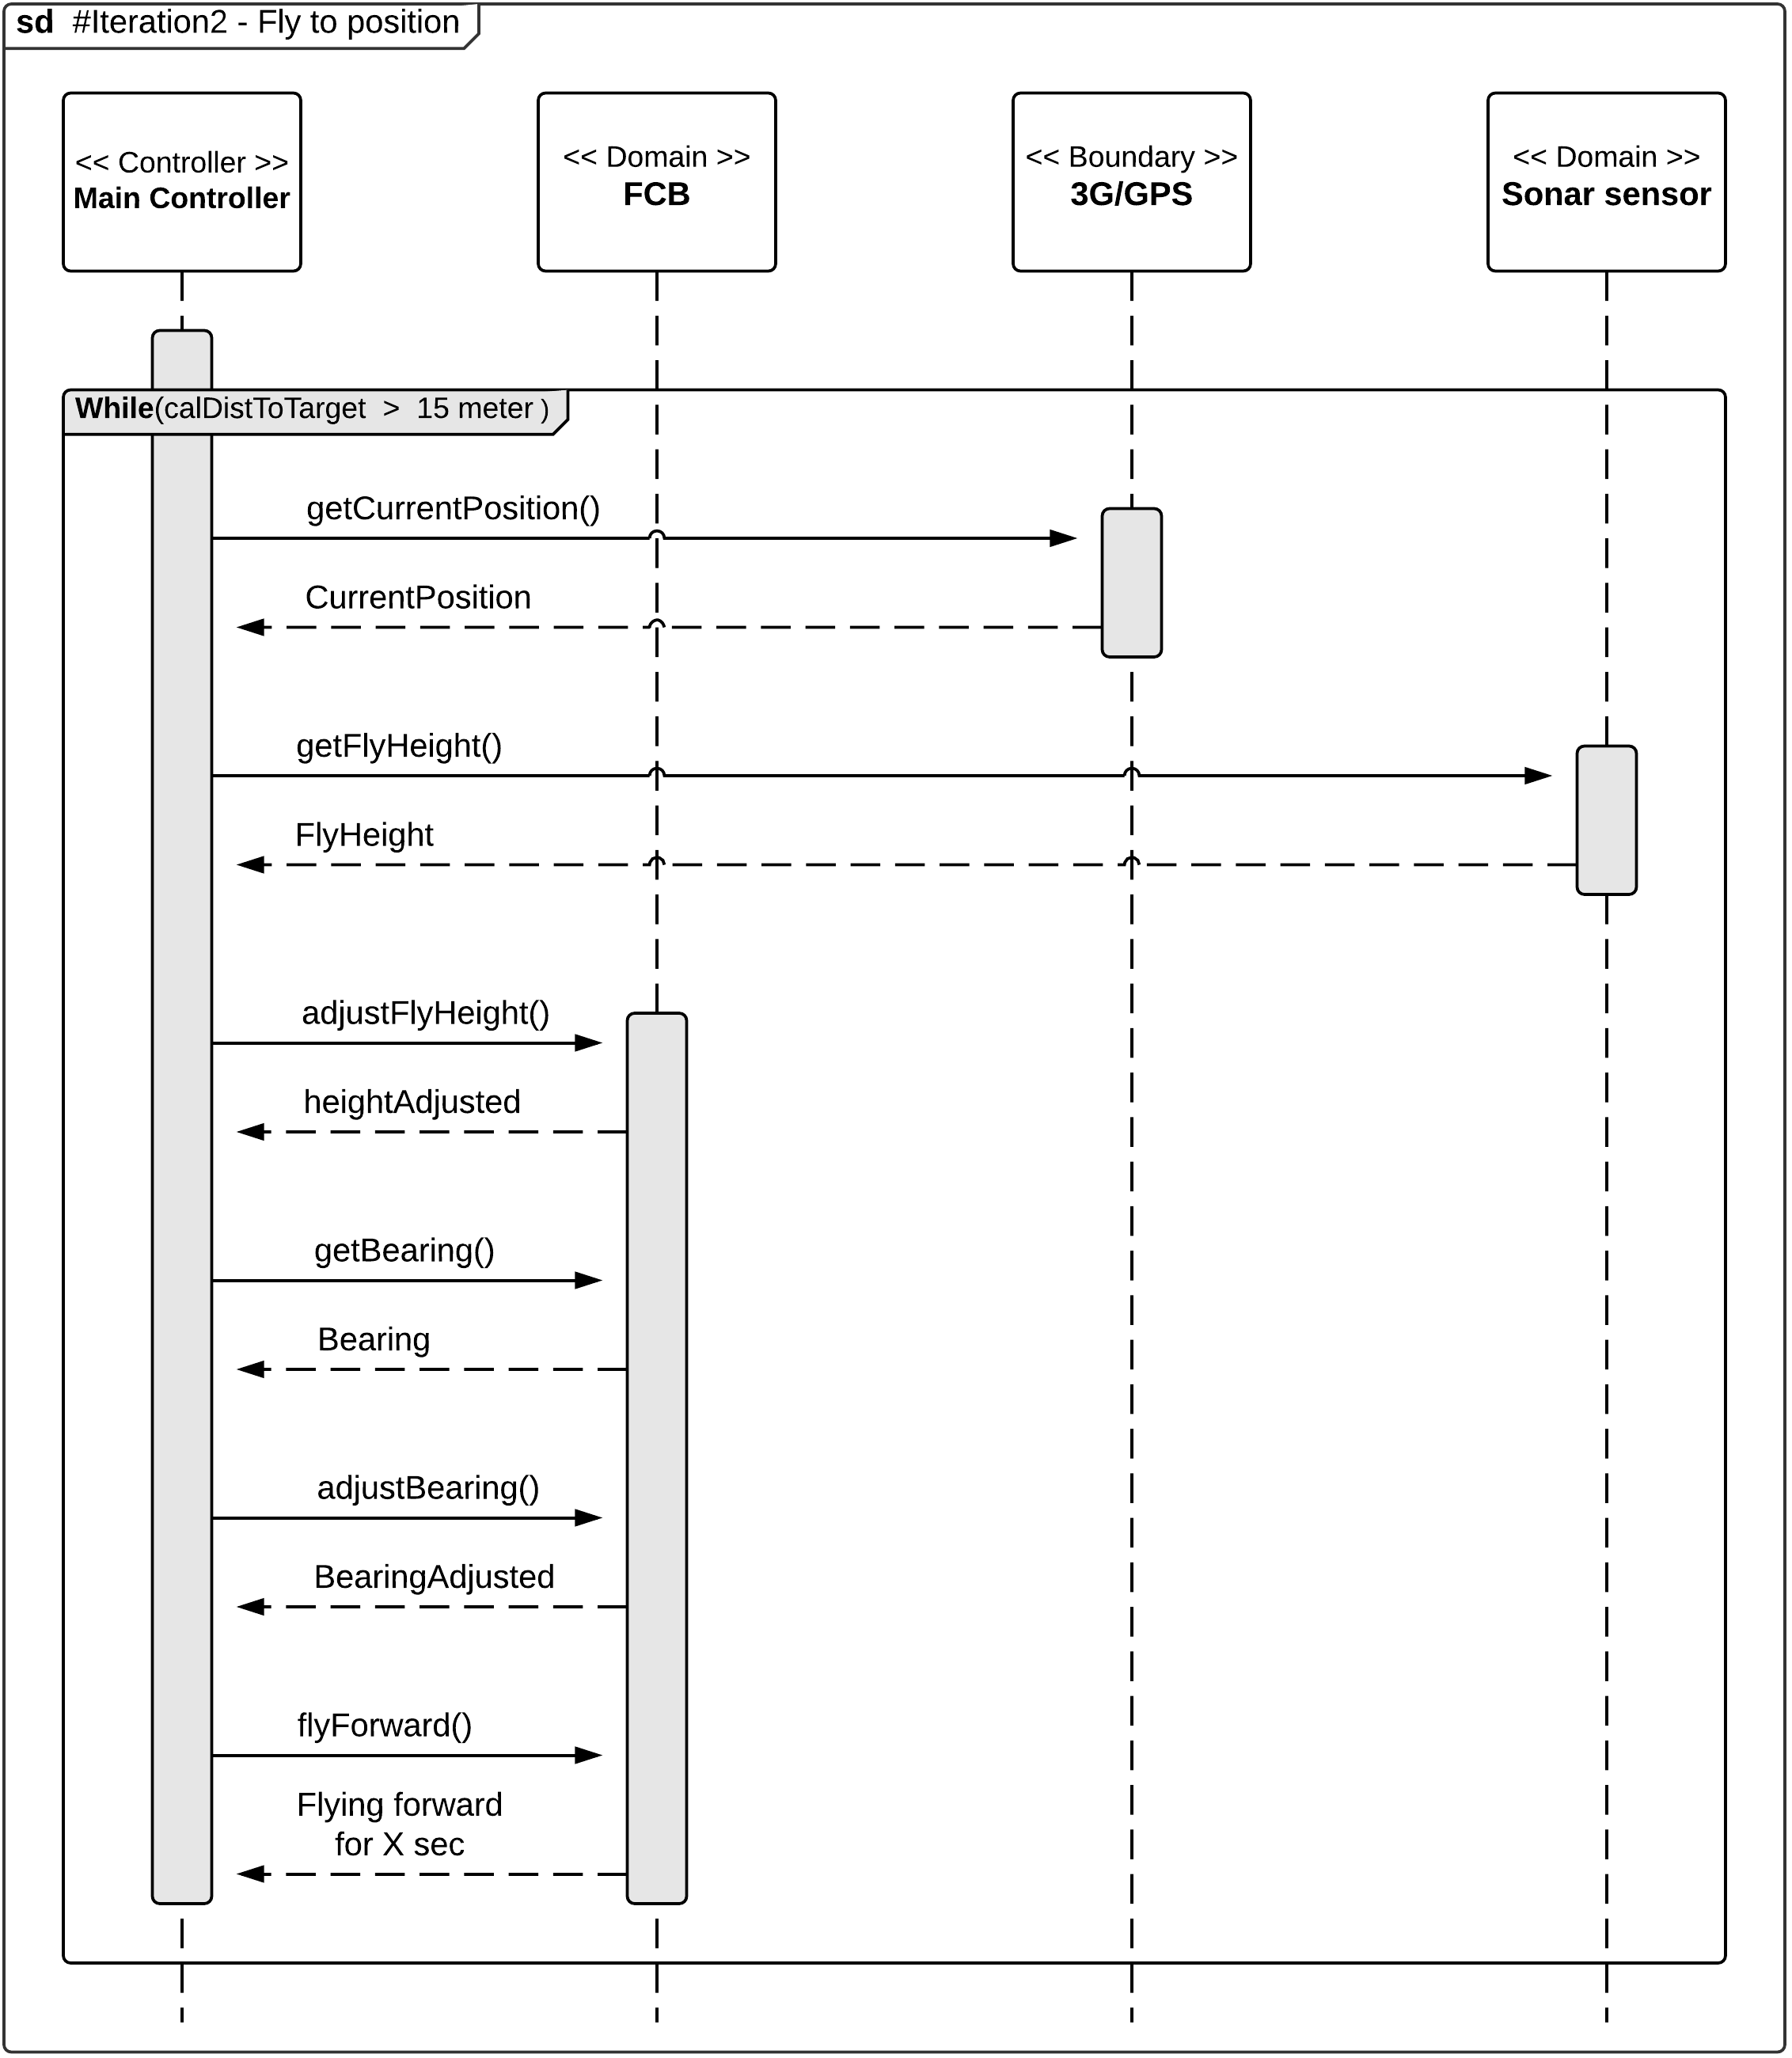
\includegraphics[width=1\textwidth]{Billeder/sekvens/sekvens_iteration2_3}
	\caption{Sekvensdiagram - Drone under flyvning}
	\label{fig:Sekvens_diagram_iteration2_3}
\end{figure}




\newpage
\subsubsection*{Sekvensdiagram webapplikation}
\vspace{-0.1cm}

Der er udformet 4 forskellige sekvensdiagrammer for webapplikationen tilhørende iteration 2. Det første sekvensdiagram viser hvordan bruger logger ind på webapplikationen og opretter en flyveopsætning. Det næste sekvensdiagram viser hvordan webapplikationen fungerer og reagerer på bruger input.


Af figur \ref{fig:Sekvens_diagram_iteration2_1} fremgår det hvordan bruger opretter en ny flyveopsætning. Det vises desuden hvilke interaktioner der foretages mellem bruger og webapplikation, samt hvordan server løbende indgår og benyttes i sekvensen. 

%kommentar
\begin{figure}[H]
	\centering
	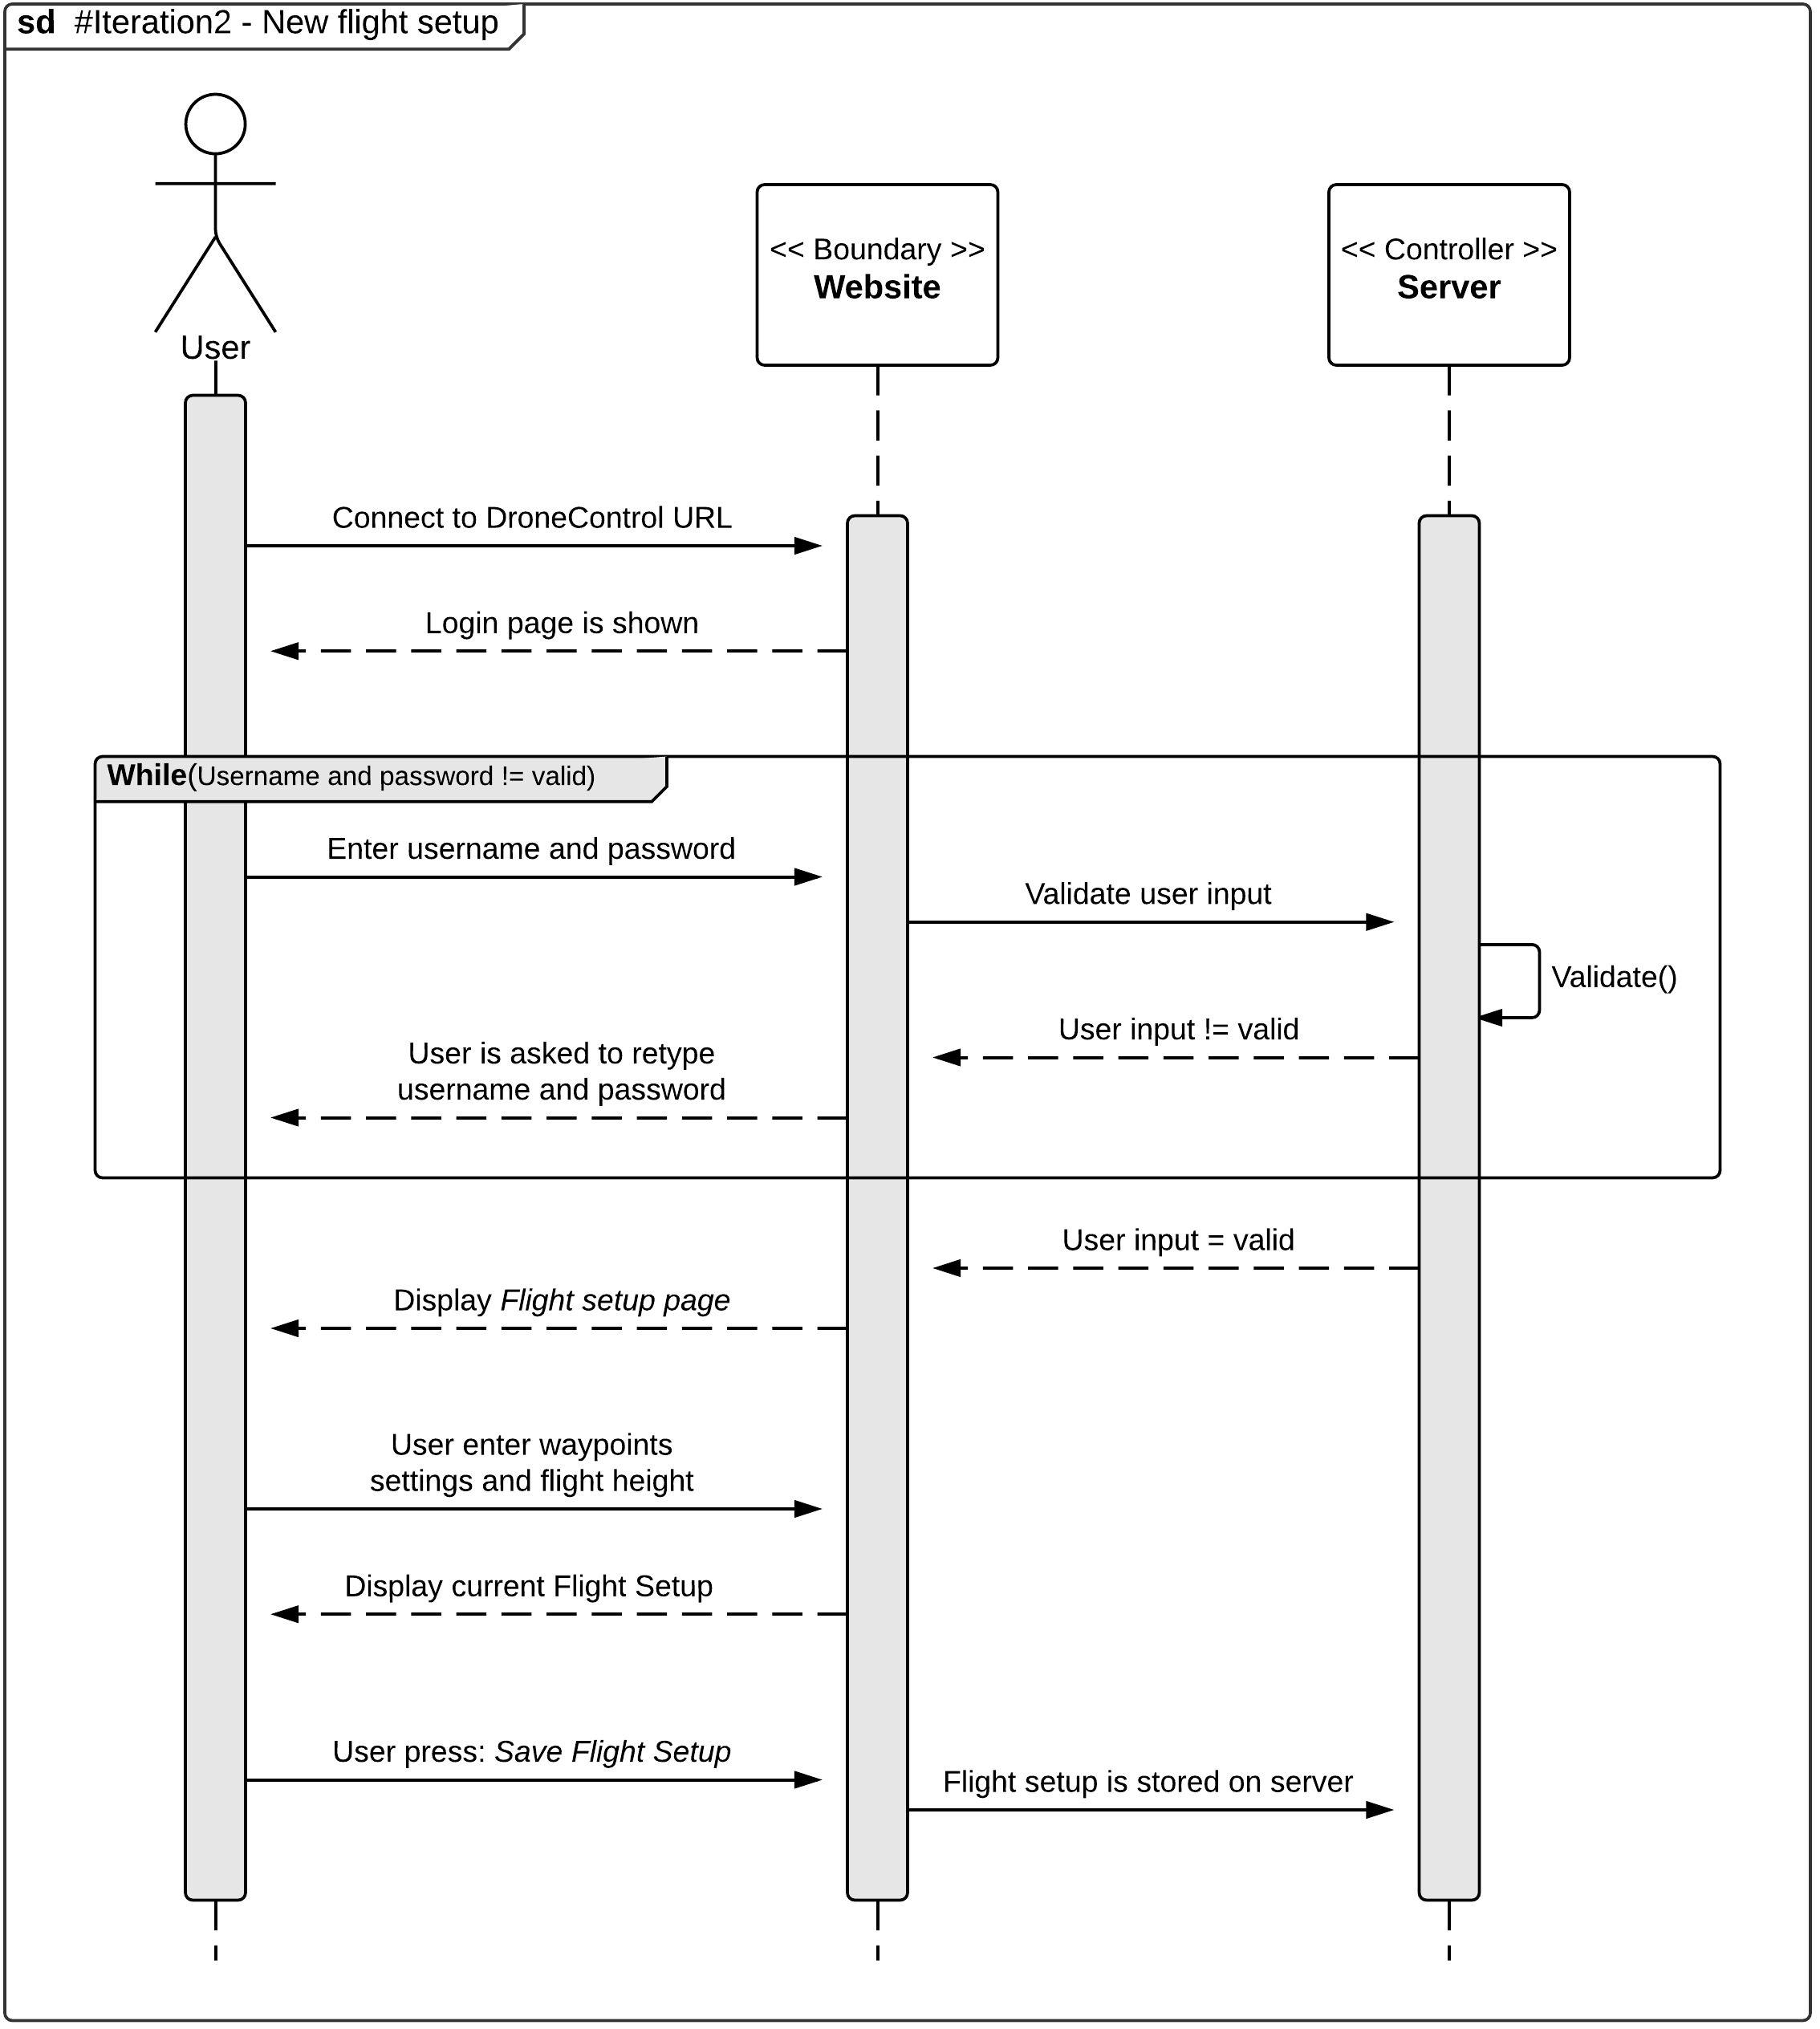
\includegraphics[width=1\textwidth]{Billeder/sekvens/sekvens_iteration2_1}
	\caption{Sekvensdiagram}
	\label{fig:Sekvens_diagram_iteration2_1}
\end{figure}


\newpage

Sekvensdiagrammet på figur \ref{fig:page_load} viser hvordan klasserne i webapplikationen interagere med hinanden ved et page load. 

\begin{figure}[H]
	\centering
	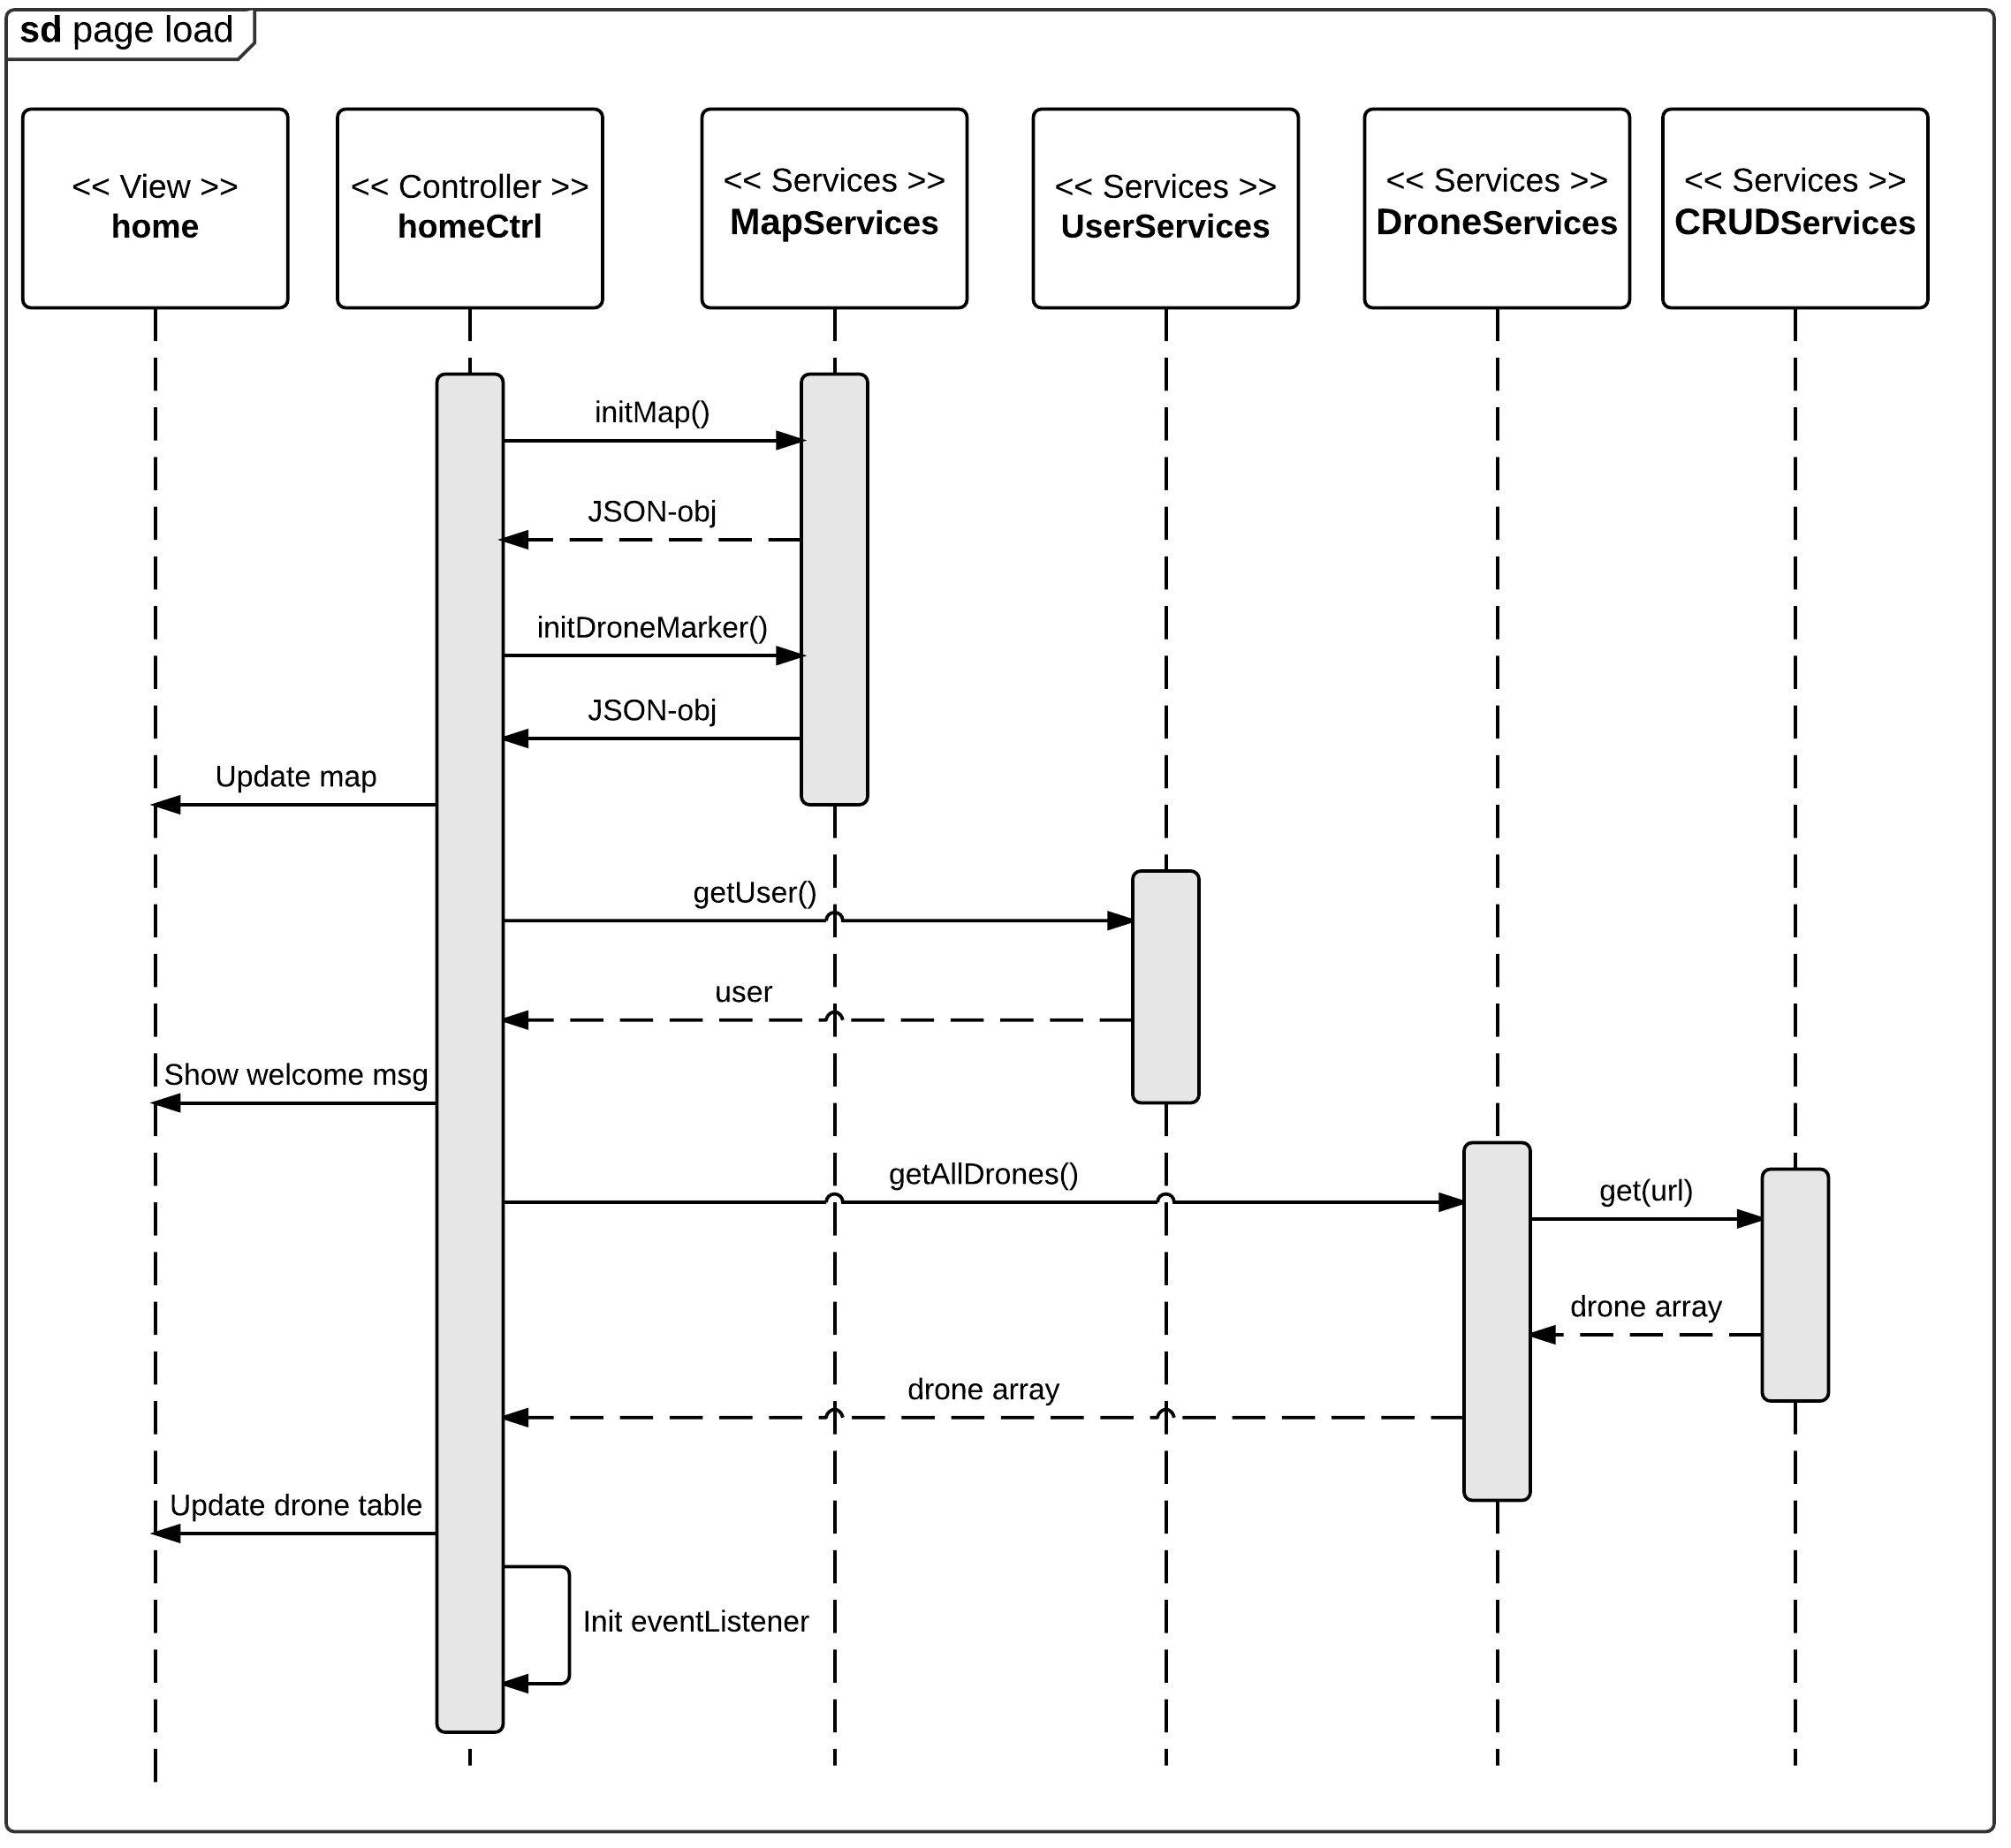
\includegraphics[width=1\textwidth]{Billeder/sekvens/sd_page_load.png}
	\caption{Sekvensdiagram page load}
	\label{fig:page_load}
\end{figure}

\newpage
På figur \ref{fig:send_waypoints} hvad der sker, når bruger gemmer en flyveopsætning. Hver service har et bestemt ansvar og de kommunikerer ud til CRUD-servicesen. Denne opbygning sikrer at logikken for data håndtering skubbes ud i diverse services. 
\begin{figure}[H]
	\centering
	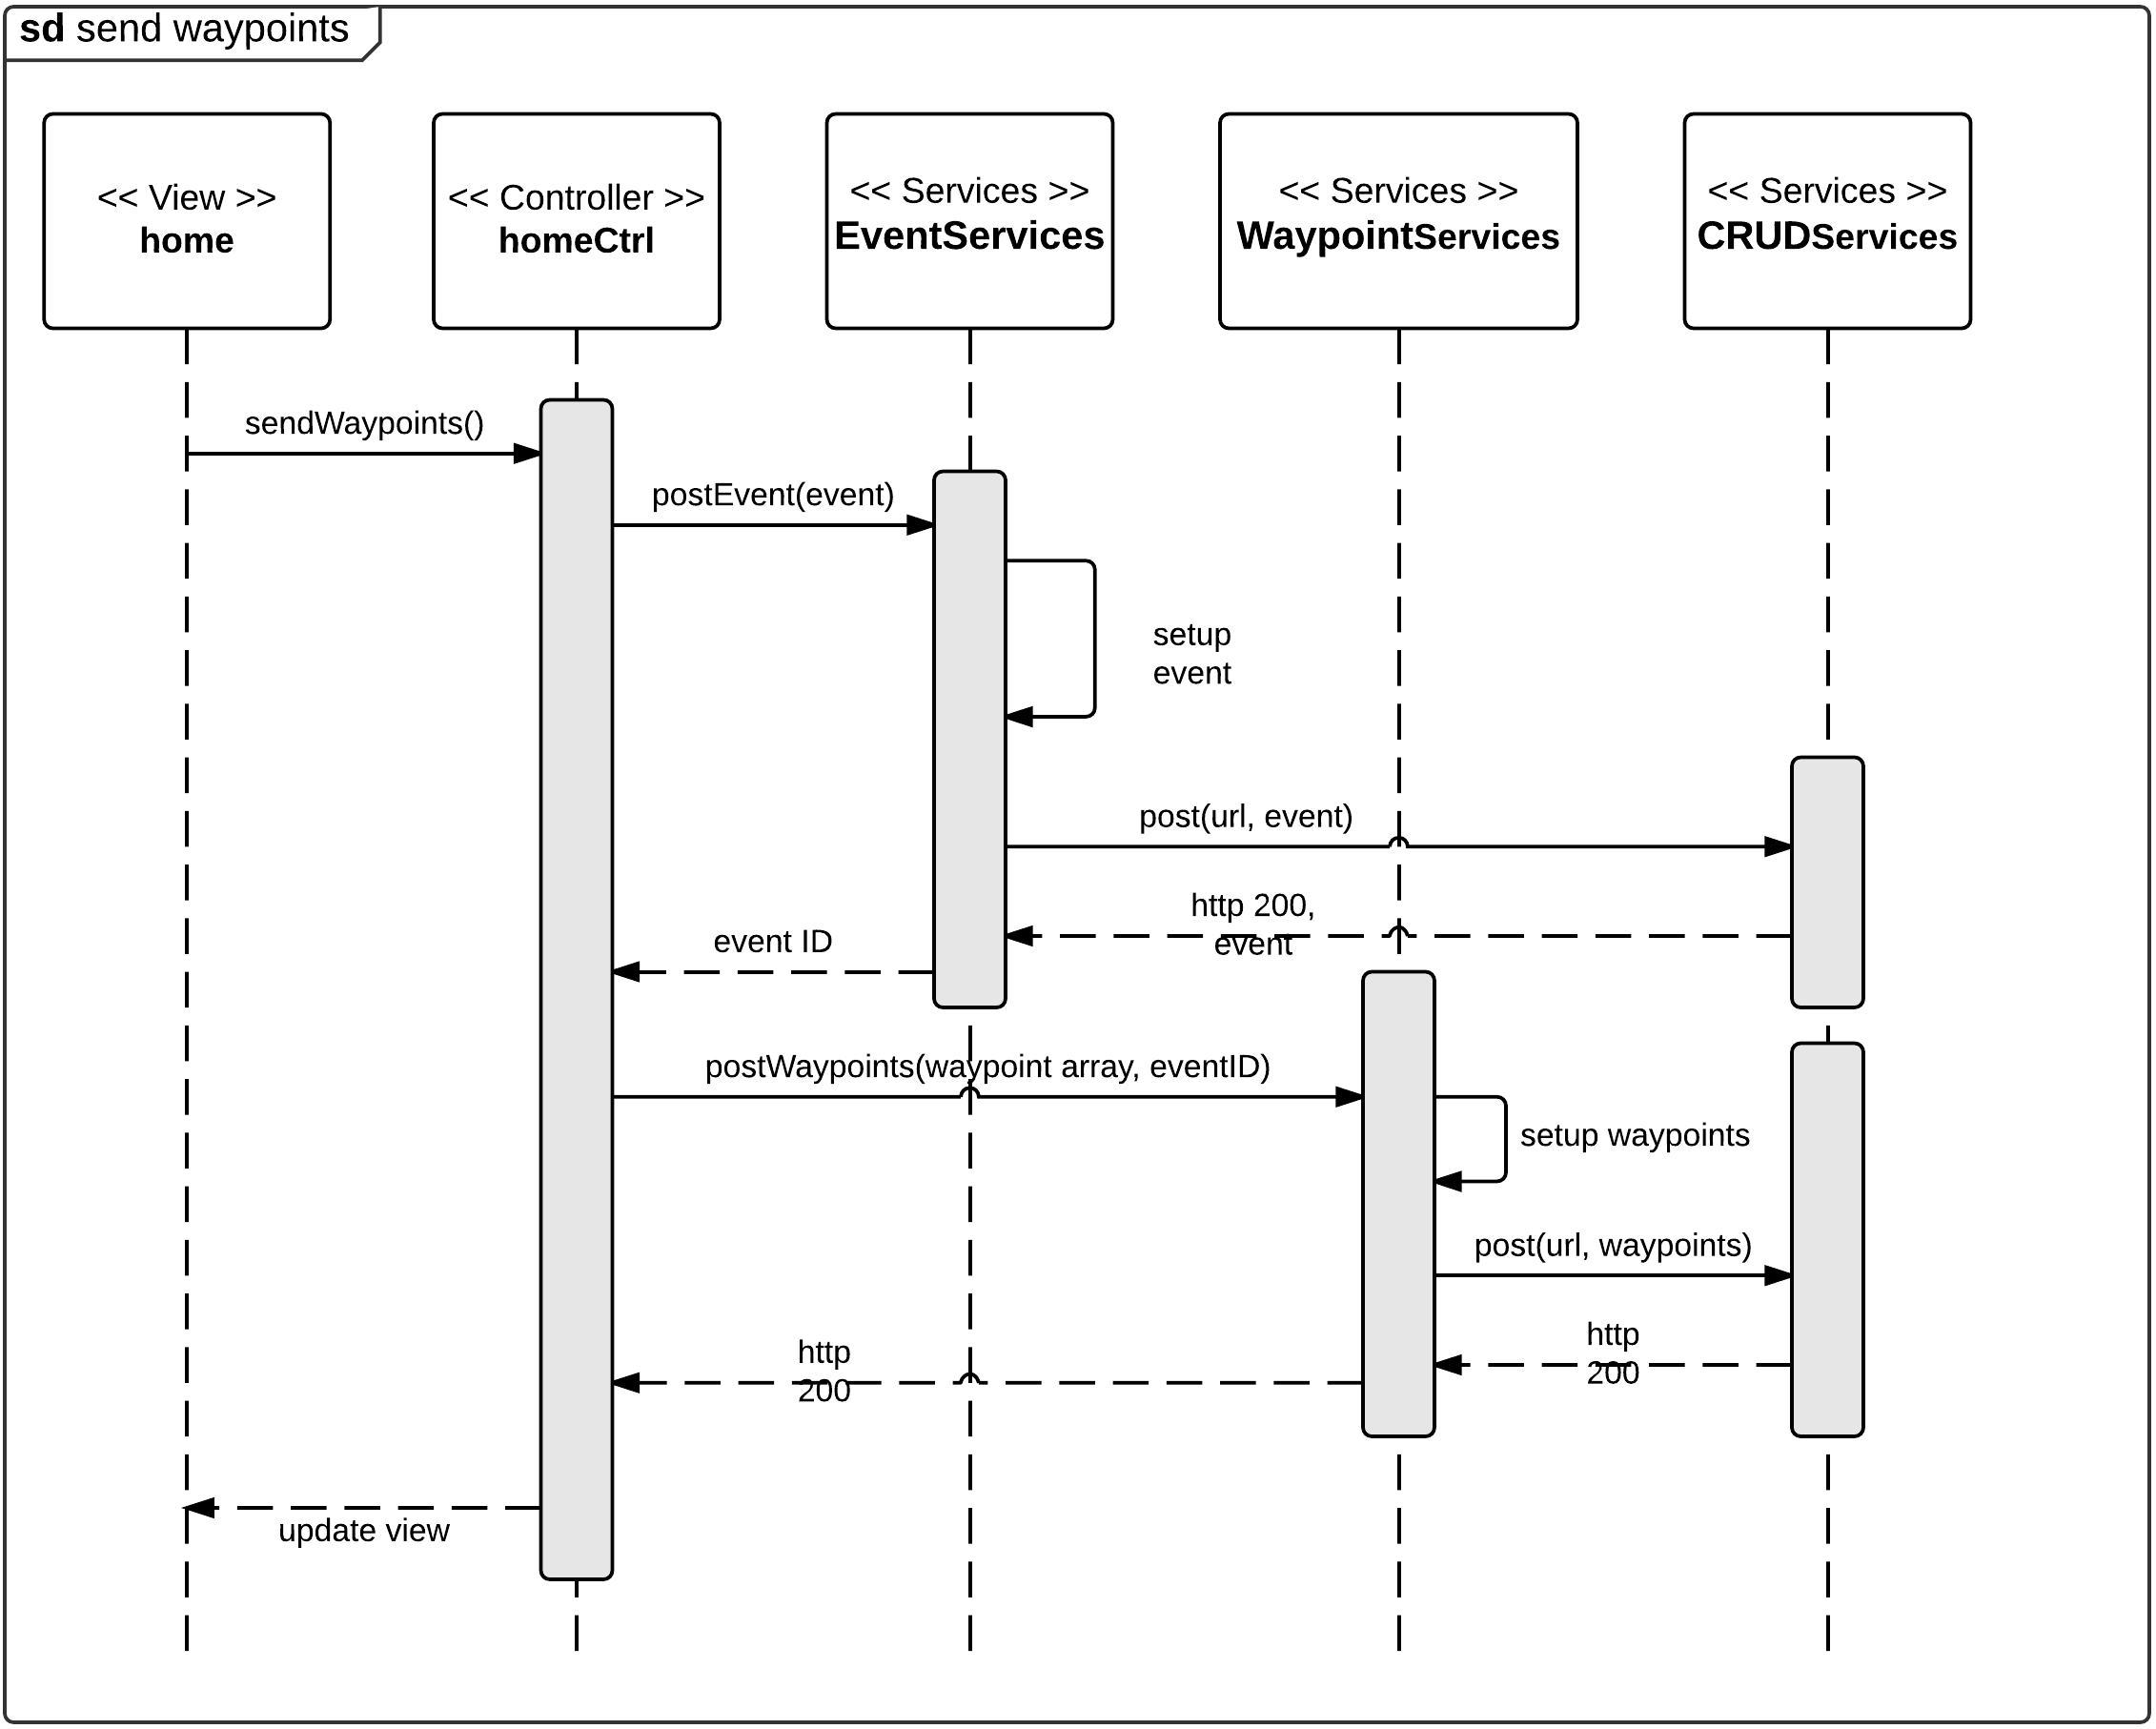
\includegraphics[width=1\textwidth]{Billeder/sekvens/sd_send_waypoints.png}
	\caption{Sekvensdiagram send waypoints}
	\label{fig:send_waypoints}
\end{figure}

\newpage
På figur \ref{fig:update_view} ses hvilke hændelser der finder sted, når bruger trykker på forskellige droner i tabellen. 

Når et klik på tabellen finder sted, skal view'et opdateres i forhold til den givne drone. Har dronen et event, skal eventet og dertilhørende waypoints vises. Hvis der ikke er noget event tilknyttet dronen, får bruger mulighed for at oprette et nyt.
\begin{figure}[H]
	\centering
	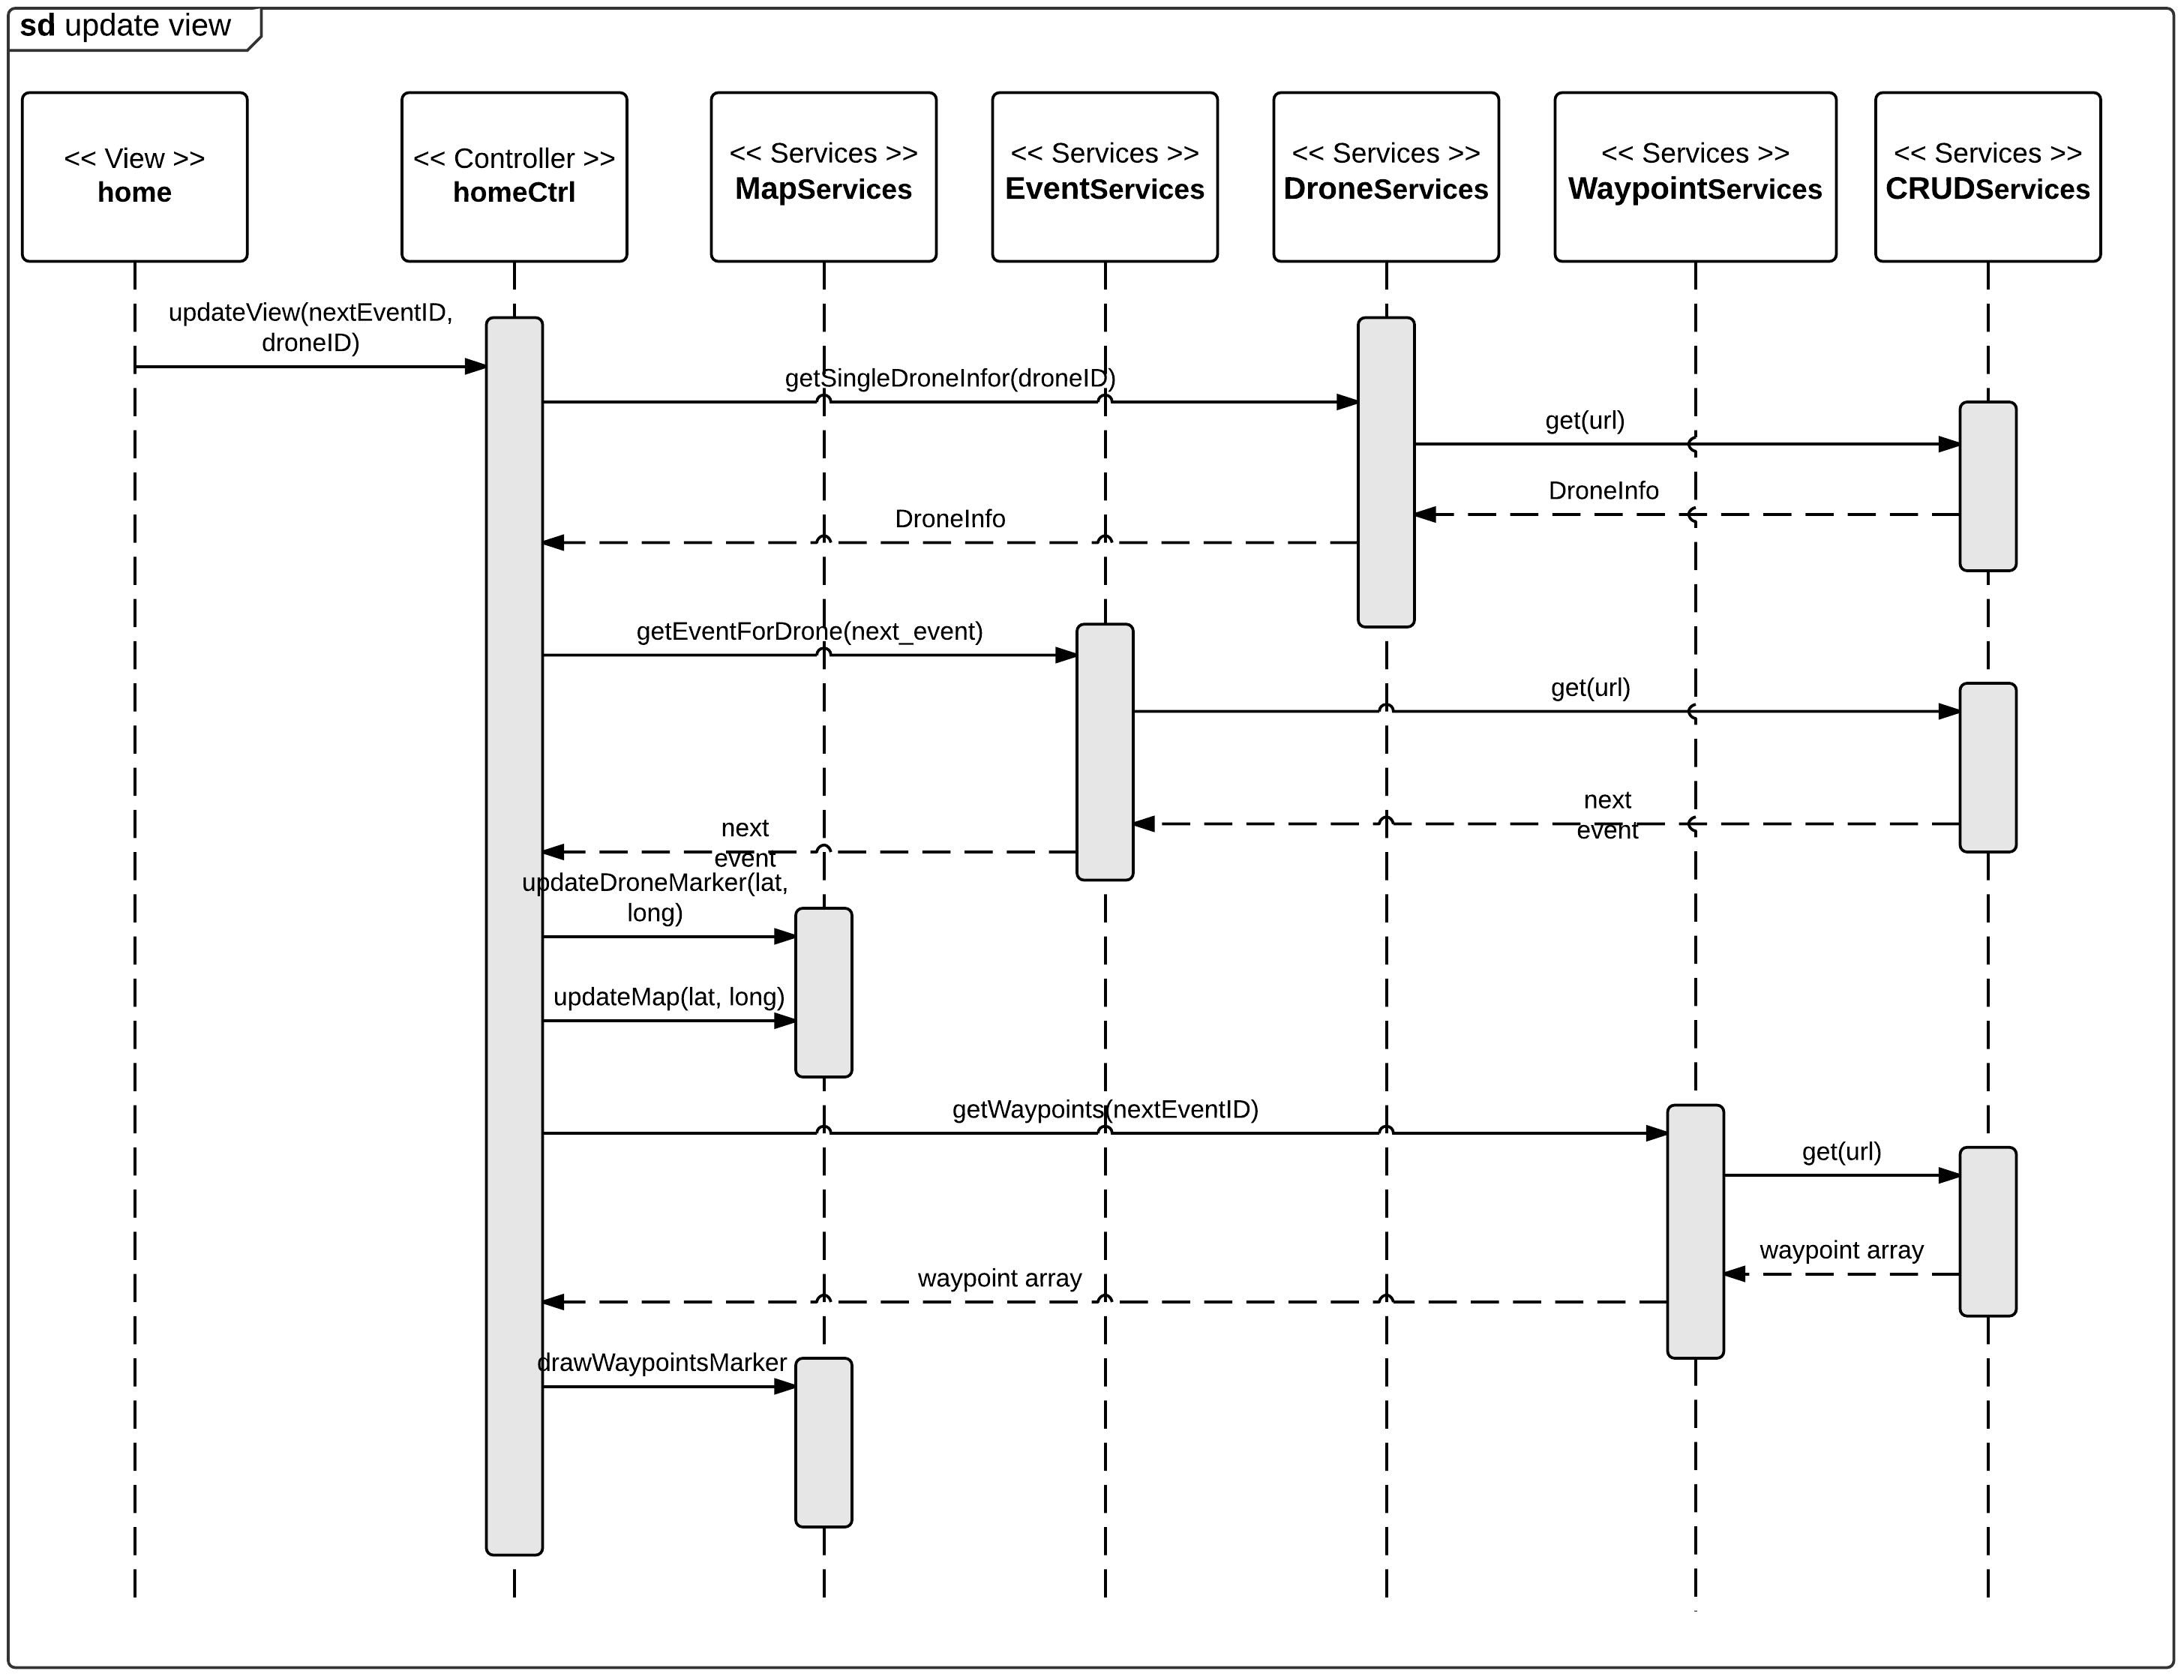
\includegraphics[width=1\textwidth]{Billeder/sekvens/sd_update_view.png}
	\caption{Sekvensdiagram opdater }
	\label{fig:update_view}
\end{figure}

\newpage
\subsubsection*{Klassediagram drone}

På figur \ref{fig:classDiagram_drone_underflyvning} ses klassediagrammet for drone. I det følgende findes en forklaring af klasserne og deres ansvarsområder. 

\begin{figure}[H]
	\centering
	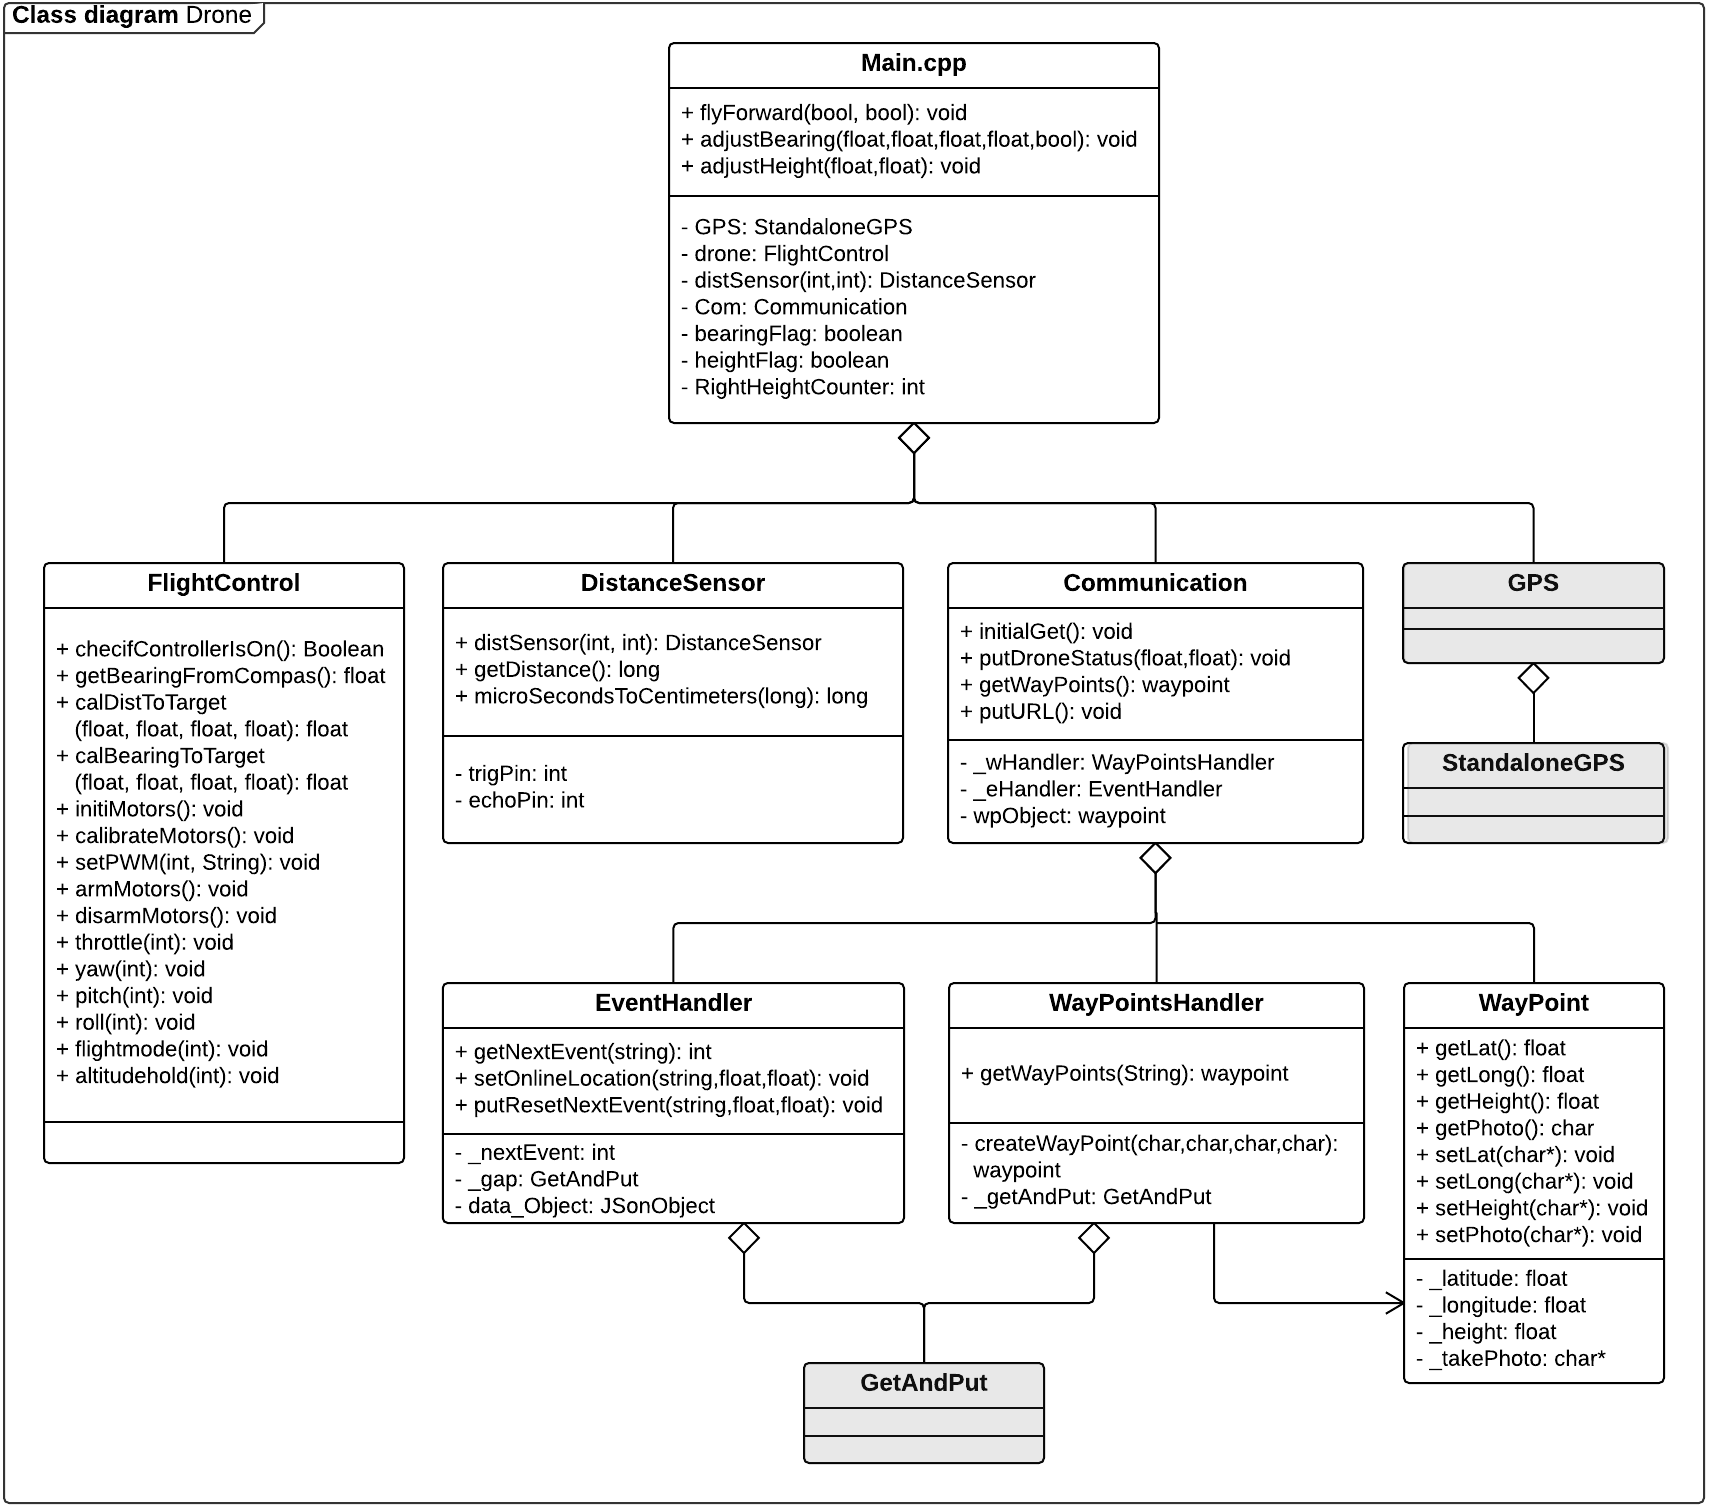
\includegraphics[width=1\textwidth]{Billeder/klasse_diagrammer/classdiagram_iteration2_drone.png}
	\vspace{-0.7cm}
	\caption{Klassediagram drone}
	\label{fig:classDiagram_drone_underflyvning}
\end{figure}

\textbf{FlightControl} \\
FlightControl klassen står for alt styring af dronen. Bla. står FlightControl for kalibrering og styring af motorerne, samt aflæsning af højdesensor, GPS og kompas. 

\textbf{DistanceSensor} \\
DistanceSensor klassen bruges til at kontrollere de sensorer der er monteret på dronen. DistanceSensor klassen bruges udelukkende til kontrol af sensore til højdemåling. 

\textbf{WayPointsHandler} \\
WayPointsHandler klassen håndterer de waypoints der hentes ned fra server. Klassen tager de hentede waypoints og gør dem tilgængelige for main.cpp. WayPointsHandleren gør brug af set-metoder fra WayPoint klassen.

\textbf{WayPoint} \\
WayPoint klassen bruges til at hente waypoints.  

\textbf{Main.cpp} \\
Main.cpp filen bruges til at sætte arduino board korrekt op, bla. sættes baudrate på de forskellige serielle forbindelser. Desuden bruges Main.cpp til at kalde og eksekverer forskellige klasse, objekter og funktioner.

\textbf{GPS} \\
GPS klassen er implementeret som en abstract klasse. Init og updateGPSPosition er lavet som virtuelle metoder, hvilket betyder de skal implementeres i alle afledte klasser. GPS klassen er lavet fordi 3G/GPS modulet kunne bruges i 3 forskellige GPS modes. 

\textbf{StandaloneGPS}\\
Denne klasse er ansvarlig for al kommunikation med GPS'en når standalone mode er valgt. 

\textbf{GetAndPut} \\
GetAndPut klassen er den klasse der er tættest på hardwaren. Klassen indeholder http metoder der bruges til kommunikation mellem dronen og serveren. 

\textbf{Communication} \\
Communication klassen styrer alt der har med 3G kommunikation at gøre.

\textbf{EventHandler} \\
EventHandler klassen håndterer Events, og bruges som bindeled mellem communication- og GetAndPut klassen. EventHandleren sorterer eventID'et fra data der modtages og returnerer værdien af eventID til communication klassen. 

\newpage


\subsubsection*{Klassediagram webapplikation}
\vspace{-0.1cm}
På figur \ref{fig:classDiagram_home} ses klasse diagrammet tilhørende iteration 2 for websitet. Funktionaliteten af systemet er blevet udvidet, så der nu er overblik over droner i systemet og deres status. Desuden er der mulighed for at oprette events til bestemte droner. 
\begin{figure}[H]
	\centering
	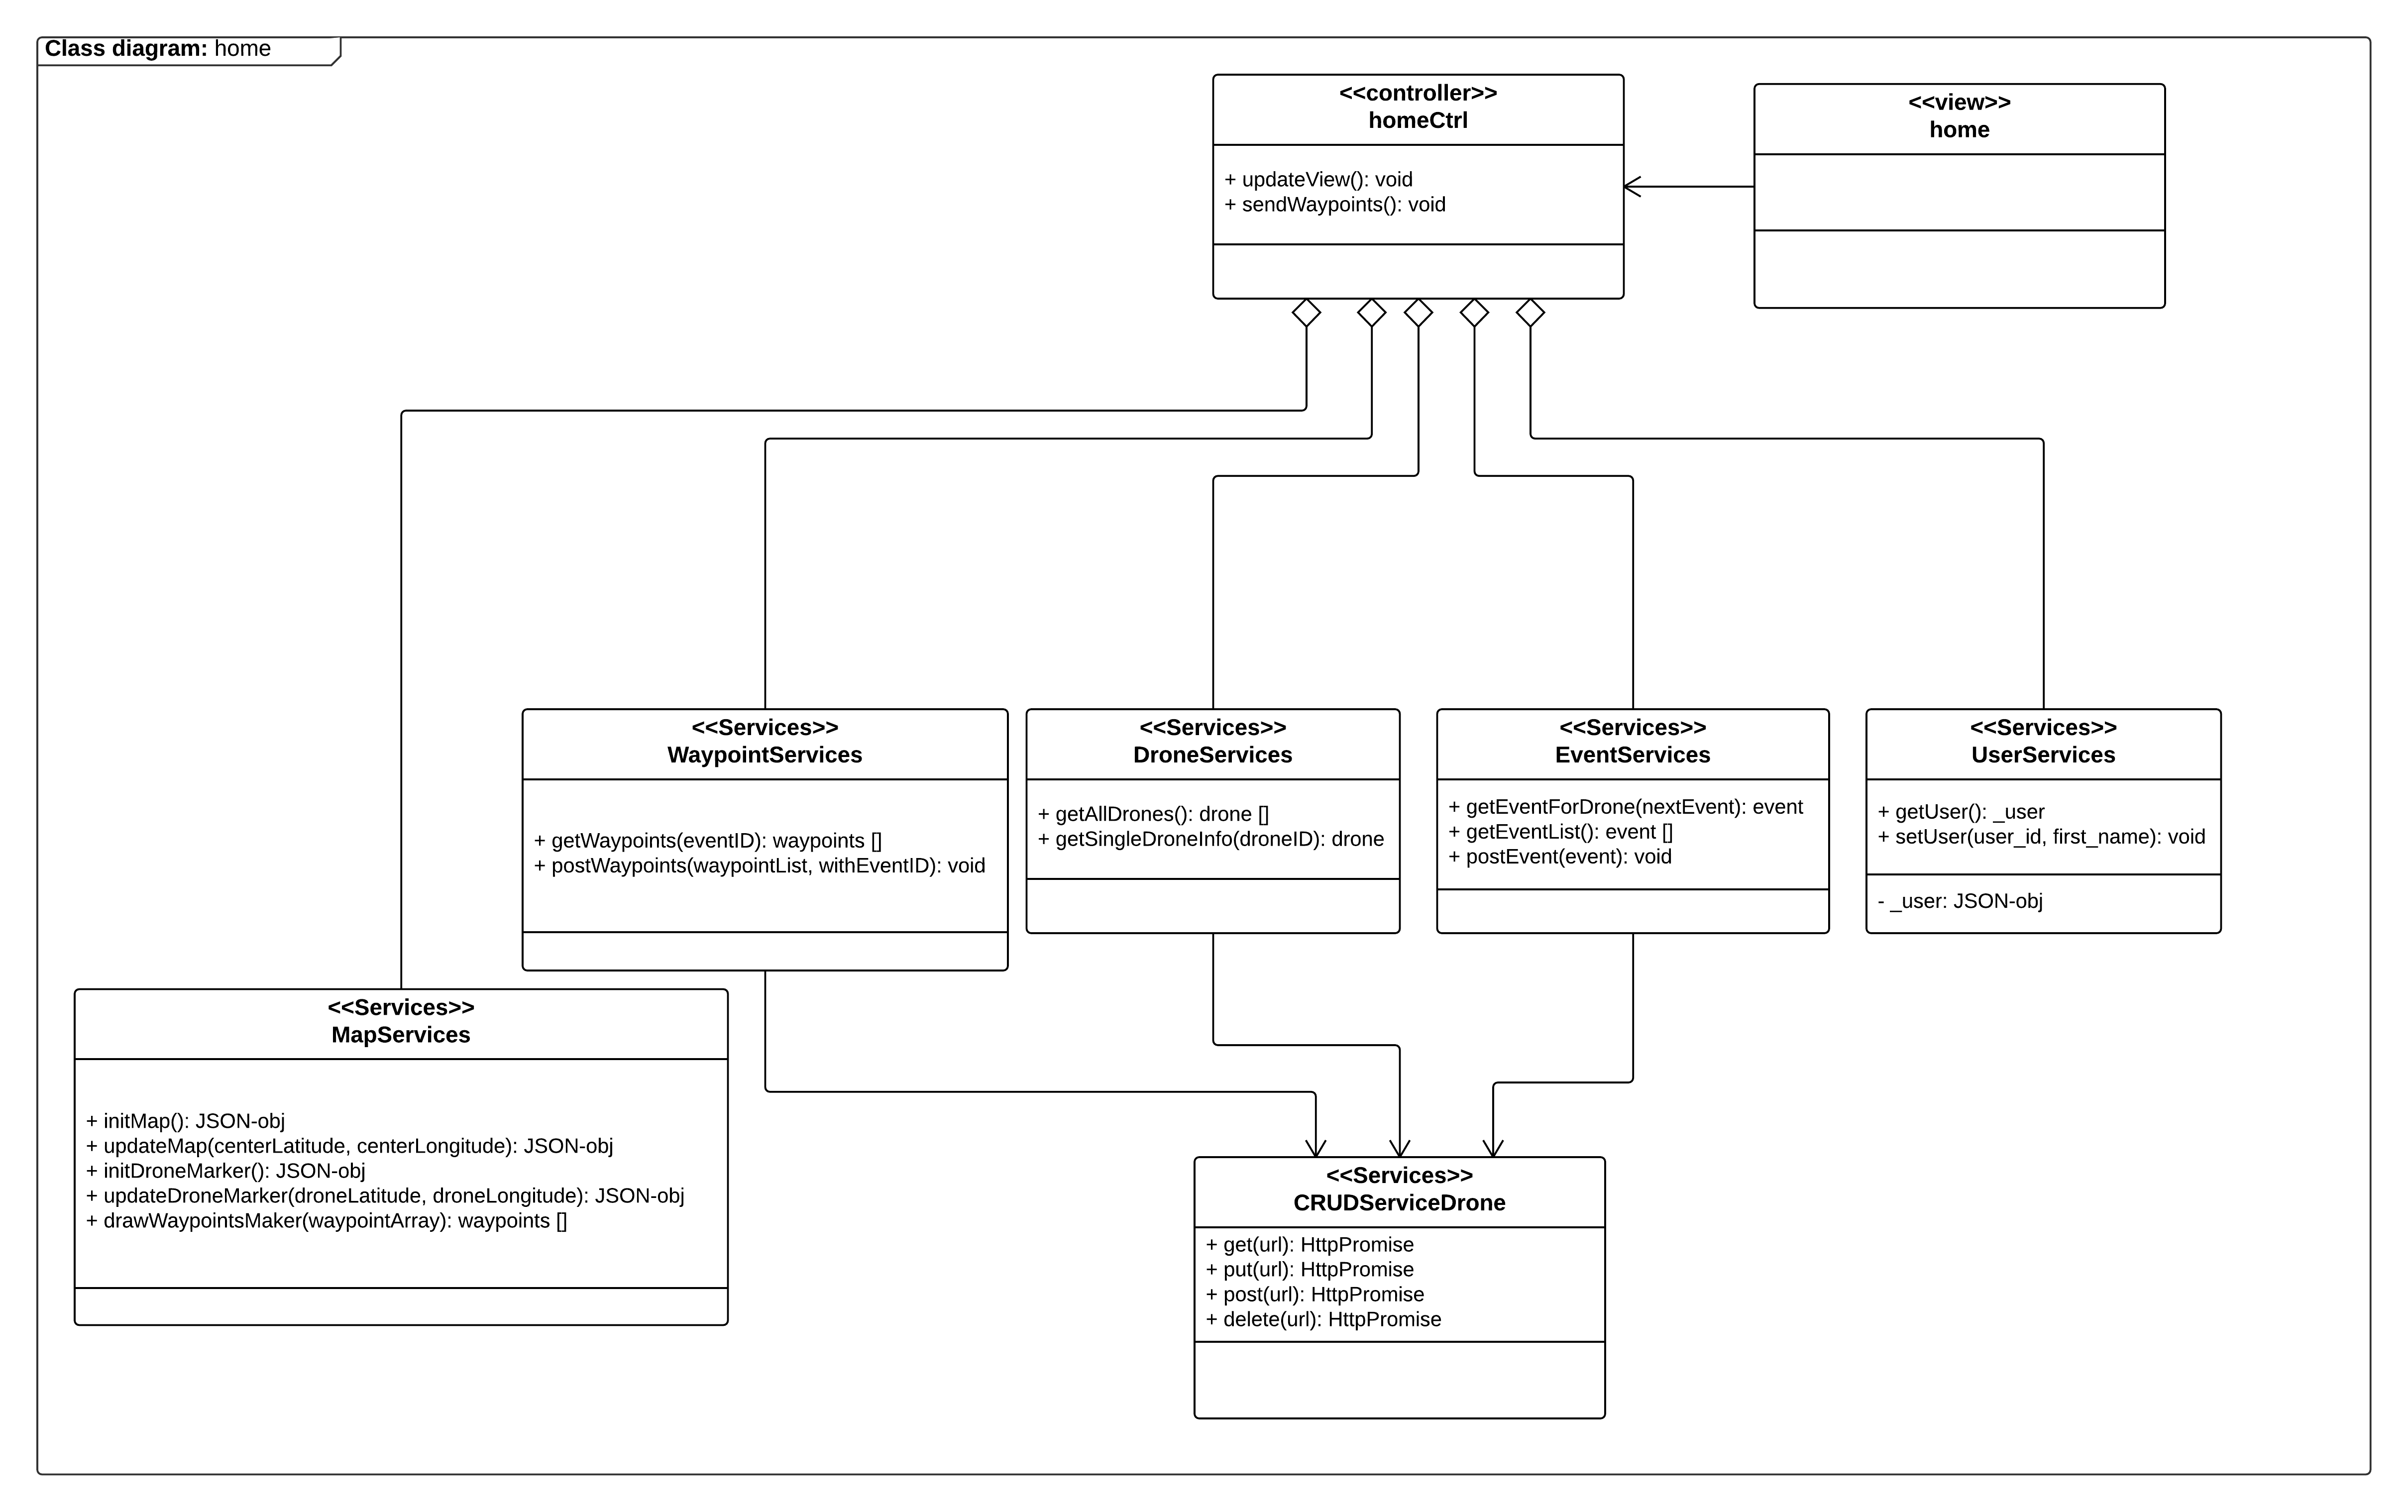
\includegraphics[width=1.\textwidth]{Billeder/klasse_diagrammer/home_class_diagram.png}
	\vspace{-0.5cm}
	\caption{Klassediagram home}
	\label{fig:classDiagram_home}
\end{figure}

\textbf{home}
Denne klasse er view'et tilhørende iteration to. Denne klasse sammen med homeCtrl skaber det endelig view som brugeren ser i sin browser når han besøger siden.

\textbf{homeCtrl}
HomeCtrl klassen er controller klassen til iteration to. Det er den eneste klasse der har direkte forbindelse til view'et, homeCtrl klassen deler også hukommelse med view'et igennem two-way-binding med scopes.

\textbf{DroneServices}
Denne klasse indeholder logikken om drone håndteringen. Den har ansvaret for at hente informationer omkring droner fra serveren via CRUDServiceDrone klassen.

\textbf{WaypointServices}
Denne klasse indeholder logikken om waypoint håndtering. Denne klasse henter henter waypoints tilhørende et event til controller klassen. Klassen bliver også brugt til at sende waypoints til serveren via CRUDServiceDrone klassen.

\textbf{EventServices}
Denne klasse indeholder logikken om event håndtering. Klassen bruges til at hente en event liste, et enkelt event for en givet drone og sende et nyoprettet event til serveren via CRUDServiceDrone klassen.

\textbf{MapServices}
Denne klasse indeholder logikken om map håndtering. Klassen bruges til at opdatere kortet i view'et, tegne waypoints og dronen på kortet.


\newpage

\textbf{CRUDServicesDrone}
Denne klasse bruges som bindeled imellem server og webapplikation, og indeholder logik til serveren. CRUDServicesDrone bruges når der sendes Get, Put og Post til serveren.

\textbf{UserServices}
Denne klasse blev oprettet i iteration et og bruges til at gemme information omkring hvilke bruger der er logget ind i systemet.

\vspace{1cm}

\subsubsection*{State machine diagram}
\vspace{-0.1cm}
I state machine diagrammet på figur \ref{fig:Statemachine_iteration2}, vises de forskellige states der eksisterer til iteration 2 og hvordan flowet imellem dem ser ud. 
%kommentar
\begin{figure}[H]
	\centering
	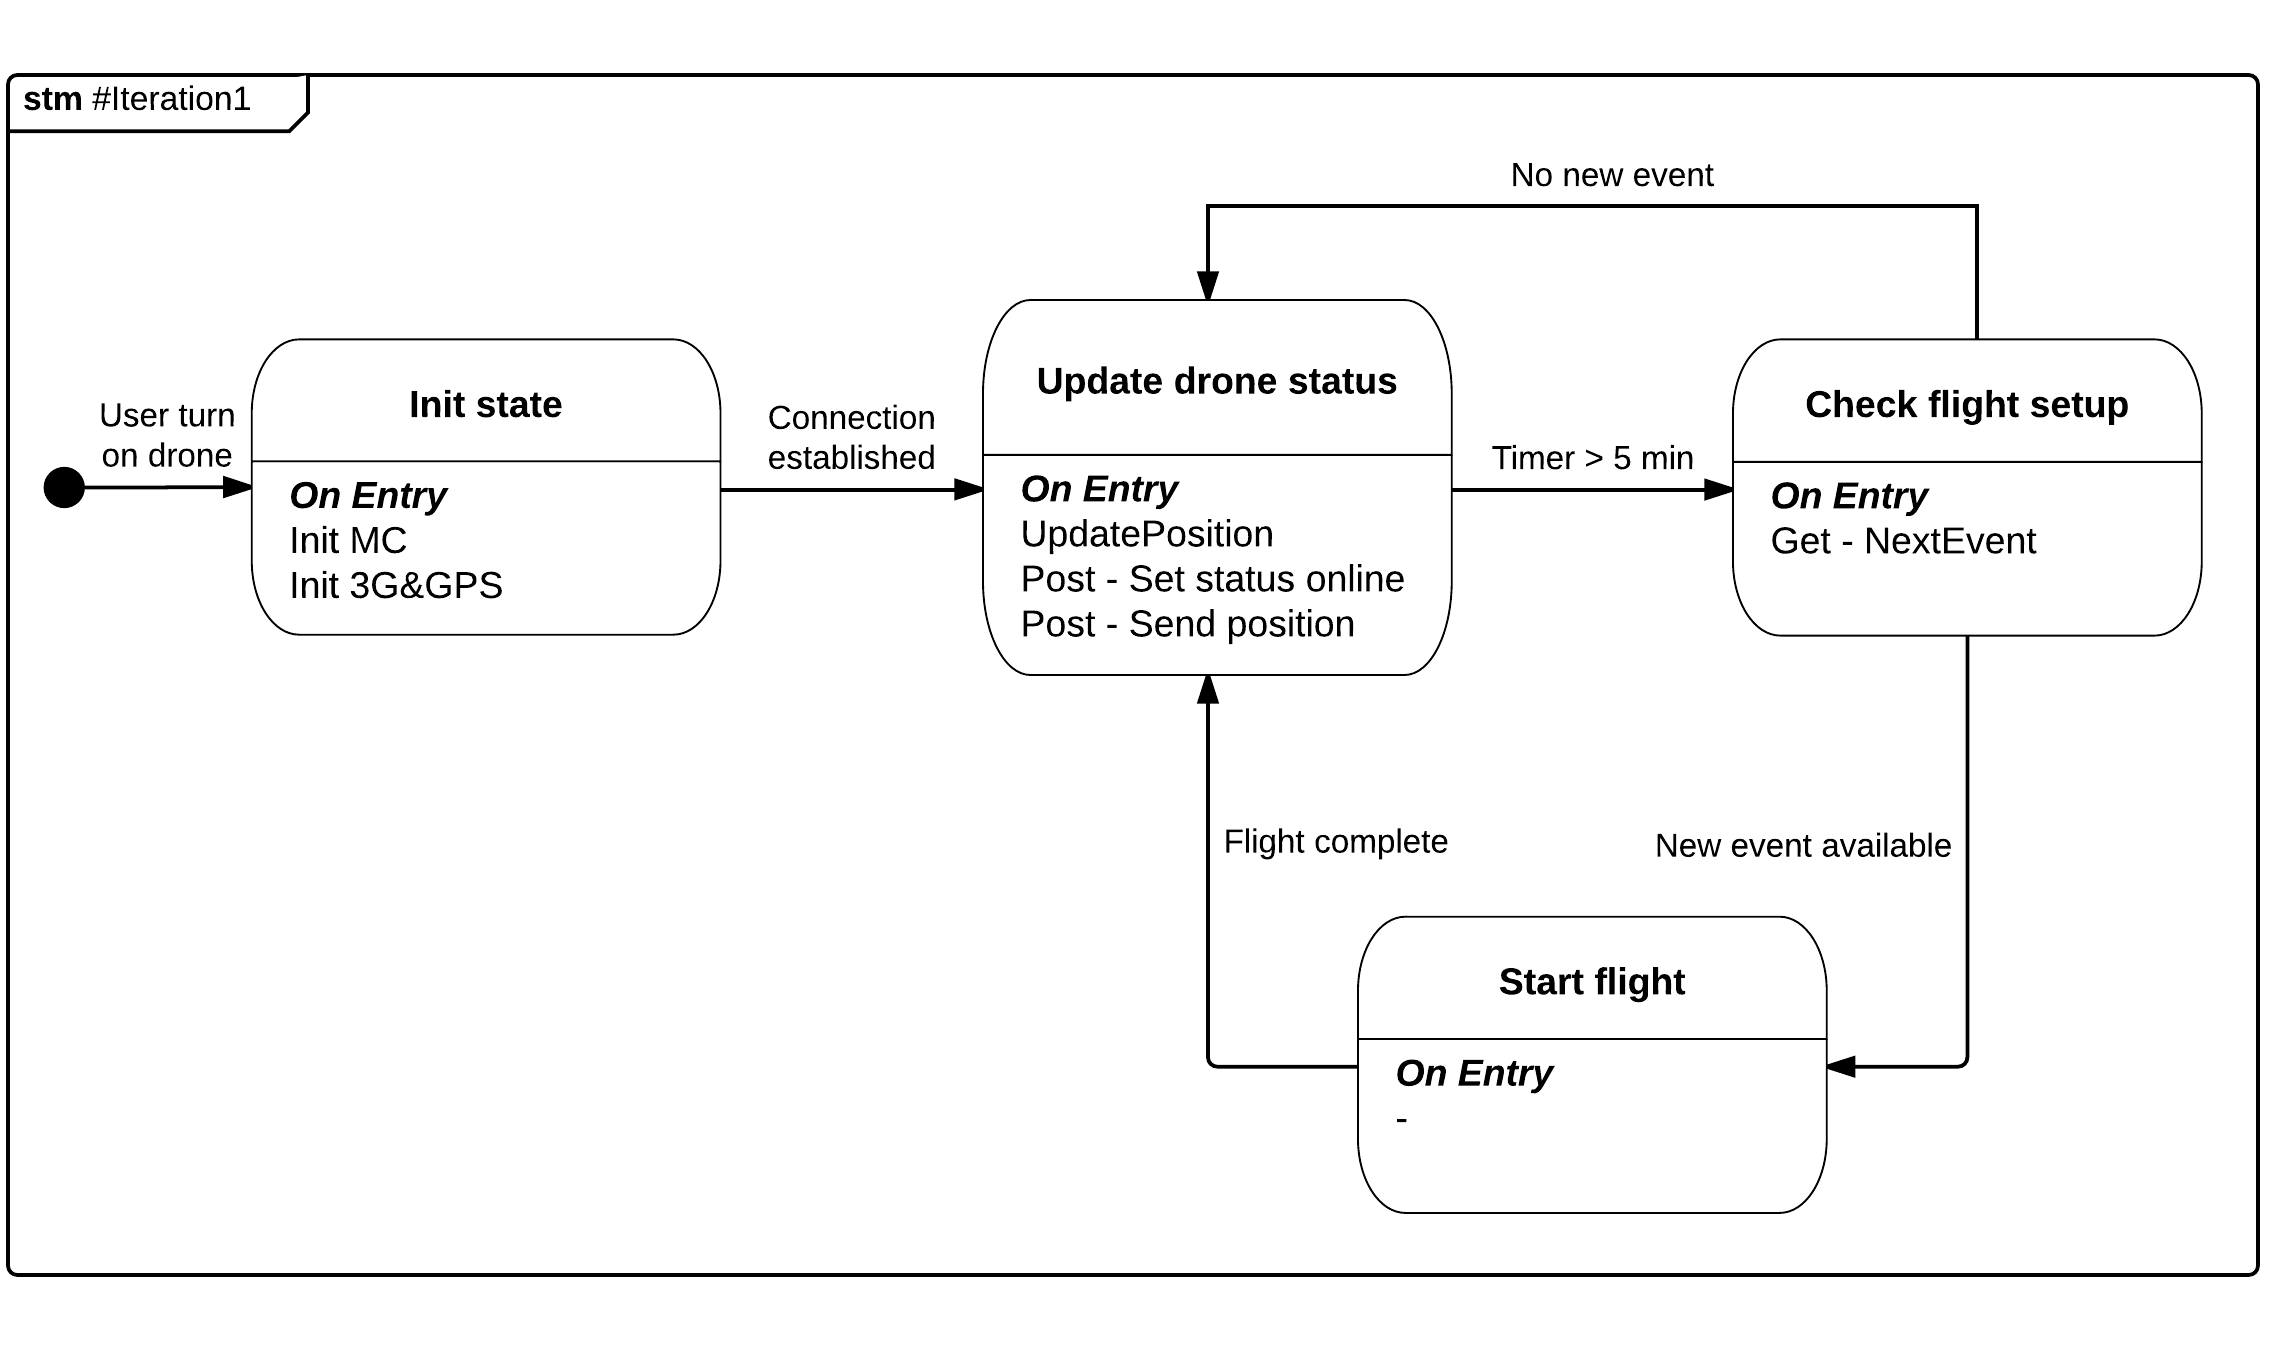
\includegraphics[width=1\textwidth]{Billeder/statemachine/State_iteration2.png}
	\vspace{-0.5cm}
	\caption{State machine \#iteration 2}
	\label{fig:Statemachine_iteration2}
\end{figure}